\documentclass[12pt]{article}
\usepackage[letterpaper,left=0.7in,right=0.7in,top=0.85in,bottom=0.85in,
  headheight=16pt,headsep=12pt,footskip=26pt]{geometry}
\usepackage[T1]{fontenc}
\usepackage{tgheros}
\renewcommand{\familydefault}{\sfdefault}
\usepackage{xcolor}
\usepackage{tikz}
\usetikzlibrary{arrows.meta}
\usepackage{fancyhdr}
\pagestyle{fancy}
\fancyhf{}
\lhead{\small Week 97 / Square remainders / K--1}
\lfoot{\small Bellingham Math Circle / Week 97 / W97-K-v1}
\rfoot{\small \thepage}
\renewcommand{\headrulewidth}{0pt}
\setlength{\parindent}{0pt}
\setlength{\parskip}{0pt}
\definecolor{tilefill}{RGB}{126,166,214}
\definecolor{tileline}{RGB}{40,70,115}
\definecolor{ringA}{RGB}{70,118,190}
\definecolor{ringB}{RGB}{245,205,85}
\definecolor{cardfill}{RGB}{255,246,214}
\tikzset{
  tile/.style={fill=tilefill,draw=tileline,line width=0.45pt},
  wbox/.style={draw=black,line width=0.9pt,rounded corners=1.5mm},
  lab/.style={font=\normalsize},
}
\newcommand{\prob}[1]{\textbf{Problem #1:}~}
\begin{document}
\large
Build each square on the board, filled in. To take away a group, fill the group card with tiles from the square and put them in the cup. When too few tiles are left to fill the card, those tiles are the leftover. The leftover can be 0.\par
\vspace{6mm}
{\centering 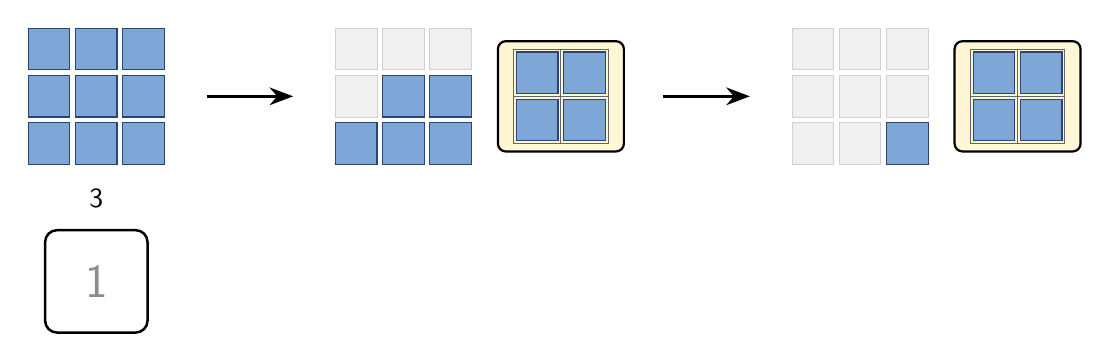
\begin{tikzpicture}[x=1mm,y=1mm]
\filldraw[tile] (0.36,0.36) rectangle (5.64,5.64);
\filldraw[tile] (0.36,6.36) rectangle (5.64,11.64);
\filldraw[tile] (0.36,12.36) rectangle (5.64,17.64);
\filldraw[tile] (6.36,0.36) rectangle (11.64,5.64);
\filldraw[tile] (6.36,6.36) rectangle (11.64,11.64);
\filldraw[tile] (6.36,12.36) rectangle (11.64,17.64);
\filldraw[tile] (12.36,0.36) rectangle (17.64,5.64);
\filldraw[tile] (12.36,6.36) rectangle (17.64,11.64);
\filldraw[tile] (12.36,12.36) rectangle (17.64,17.64);
\node[lab] at (9,-4) {3};
\draw[wbox] (2.5,-21) rectangle (15.5,-8);
\node[font=\LARGE,text=black!45] at (9,-14.5) {1};
\draw[-{Stealth[length=3mm]},line width=1pt] (23,9) -- (34,9);
\filldraw[tile] (39.36,0.36) rectangle (44.64,5.64);
\filldraw[fill=black!6,draw=black!18,line width=0.3pt] (39.36,6.36) rectangle (44.64,11.64);
\filldraw[fill=black!6,draw=black!18,line width=0.3pt] (39.36,12.36) rectangle (44.64,17.64);
\filldraw[tile] (45.36,0.36) rectangle (50.64,5.64);
\filldraw[tile] (45.36,6.36) rectangle (50.64,11.64);
\filldraw[fill=black!6,draw=black!18,line width=0.3pt] (45.36,12.36) rectangle (50.64,17.64);
\filldraw[tile] (51.36,0.36) rectangle (56.64,5.64);
\filldraw[tile] (51.36,6.36) rectangle (56.64,11.64);
\filldraw[fill=black!6,draw=black!18,line width=0.3pt] (51.36,12.36) rectangle (56.64,17.64);
\filldraw[fill=cardfill,draw=black,line width=0.8pt,rounded corners=1mm] (60,2) rectangle (76,16);
\draw[black!60,line width=0.4pt] (62,3) rectangle (68,9);
\filldraw[tile] (62.36,3.36) rectangle (67.64,8.64);
\draw[black!60,line width=0.4pt] (62,9) rectangle (68,15);
\filldraw[tile] (62.36,9.36) rectangle (67.64,14.64);
\draw[black!60,line width=0.4pt] (68,3) rectangle (74,9);
\filldraw[tile] (68.36,3.36) rectangle (73.64,8.64);
\draw[black!60,line width=0.4pt] (68,9) rectangle (74,15);
\filldraw[tile] (68.36,9.36) rectangle (73.64,14.64);
\draw[-{Stealth[length=3mm]},line width=1pt] (81,9) -- (92,9);
\filldraw[fill=black!6,draw=black!18,line width=0.3pt] (97.36,0.36) rectangle (102.64,5.64);
\filldraw[fill=black!6,draw=black!18,line width=0.3pt] (97.36,6.36) rectangle (102.64,11.64);
\filldraw[fill=black!6,draw=black!18,line width=0.3pt] (97.36,12.36) rectangle (102.64,17.64);
\filldraw[fill=black!6,draw=black!18,line width=0.3pt] (103.36,0.36) rectangle (108.64,5.64);
\filldraw[fill=black!6,draw=black!18,line width=0.3pt] (103.36,6.36) rectangle (108.64,11.64);
\filldraw[fill=black!6,draw=black!18,line width=0.3pt] (103.36,12.36) rectangle (108.64,17.64);
\filldraw[tile] (109.36,0.36) rectangle (114.64,5.64);
\filldraw[fill=black!6,draw=black!18,line width=0.3pt] (109.36,6.36) rectangle (114.64,11.64);
\filldraw[fill=black!6,draw=black!18,line width=0.3pt] (109.36,12.36) rectangle (114.64,17.64);
\filldraw[fill=cardfill,draw=black,line width=0.8pt,rounded corners=1mm] (118,2) rectangle (134,16);
\draw[black!60,line width=0.4pt] (120,3) rectangle (126,9);
\filldraw[tile] (120.36,3.36) rectangle (125.64,8.64);
\draw[black!60,line width=0.4pt] (120,9) rectangle (126,15);
\filldraw[tile] (120.36,9.36) rectangle (125.64,14.64);
\draw[black!60,line width=0.4pt] (126,3) rectangle (132,9);
\filldraw[tile] (126.36,3.36) rectangle (131.64,8.64);
\draw[black!60,line width=0.4pt] (126,9) rectangle (132,15);
\filldraw[tile] (126.36,9.36) rectangle (131.64,14.64);
\end{tikzpicture}\par}
\vspace{10mm}
\prob{1}Build each square and take away groups of~4. Circle every number a square can leave.\par
\vspace{9mm}
{\centering 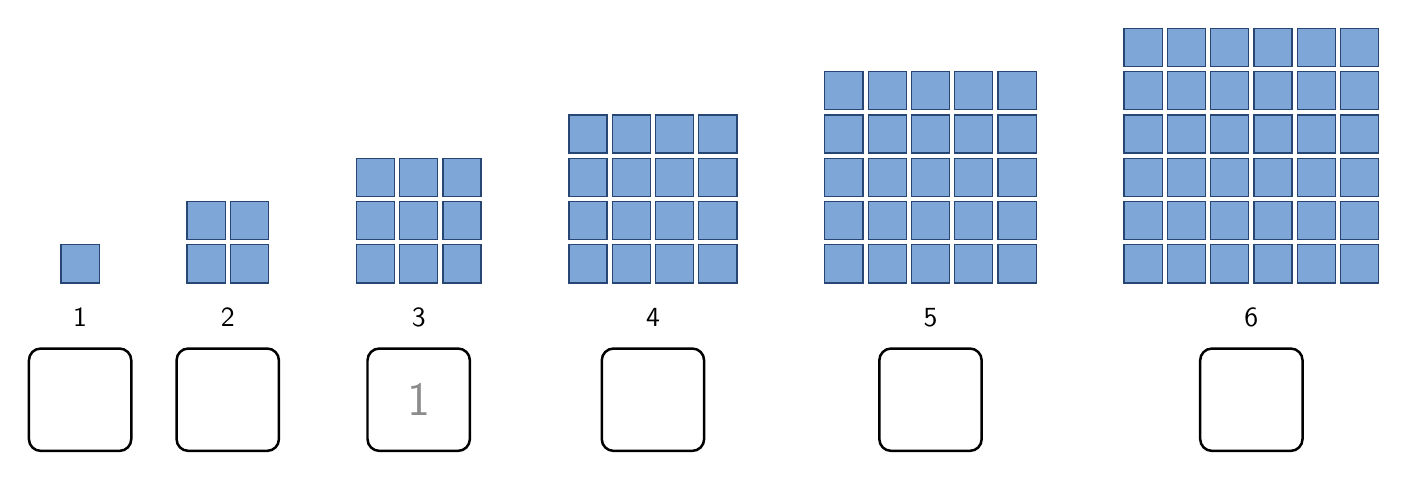
\begin{tikzpicture}[x=1mm,y=1mm]
\filldraw[tile] (0.33,0.33) rectangle (5.17,5.17);
\node[lab] at (2.75,-4) {1};
\draw[wbox] (-3.75,-21) rectangle (9.25,-8);
\filldraw[tile] (16.33,0.33) rectangle (21.17,5.17);
\filldraw[tile] (16.33,5.83) rectangle (21.17,10.67);
\filldraw[tile] (21.83,0.33) rectangle (26.67,5.17);
\filldraw[tile] (21.83,5.83) rectangle (26.67,10.67);
\node[lab] at (21.5,-4) {2};
\draw[wbox] (15,-21) rectangle (28,-8);
\filldraw[tile] (37.83,0.33) rectangle (42.67,5.17);
\filldraw[tile] (37.83,5.83) rectangle (42.67,10.67);
\filldraw[tile] (37.83,11.33) rectangle (42.67,16.17);
\filldraw[tile] (43.33,0.33) rectangle (48.17,5.17);
\filldraw[tile] (43.33,5.83) rectangle (48.17,10.67);
\filldraw[tile] (43.33,11.33) rectangle (48.17,16.17);
\filldraw[tile] (48.83,0.33) rectangle (53.67,5.17);
\filldraw[tile] (48.83,5.83) rectangle (53.67,10.67);
\filldraw[tile] (48.83,11.33) rectangle (53.67,16.17);
\node[lab] at (45.75,-4) {3};
\draw[wbox] (39.25,-21) rectangle (52.25,-8);
\node[font=\LARGE,text=black!45] at (45.75,-14.5) {1};
\filldraw[tile] (64.83,0.33) rectangle (69.67,5.17);
\filldraw[tile] (64.83,5.83) rectangle (69.67,10.67);
\filldraw[tile] (64.83,11.33) rectangle (69.67,16.17);
\filldraw[tile] (64.83,16.83) rectangle (69.67,21.67);
\filldraw[tile] (70.33,0.33) rectangle (75.17,5.17);
\filldraw[tile] (70.33,5.83) rectangle (75.17,10.67);
\filldraw[tile] (70.33,11.33) rectangle (75.17,16.17);
\filldraw[tile] (70.33,16.83) rectangle (75.17,21.67);
\filldraw[tile] (75.83,0.33) rectangle (80.67,5.17);
\filldraw[tile] (75.83,5.83) rectangle (80.67,10.67);
\filldraw[tile] (75.83,11.33) rectangle (80.67,16.17);
\filldraw[tile] (75.83,16.83) rectangle (80.67,21.67);
\filldraw[tile] (81.33,0.33) rectangle (86.17,5.17);
\filldraw[tile] (81.33,5.83) rectangle (86.17,10.67);
\filldraw[tile] (81.33,11.33) rectangle (86.17,16.17);
\filldraw[tile] (81.33,16.83) rectangle (86.17,21.67);
\node[lab] at (75.5,-4) {4};
\draw[wbox] (69,-21) rectangle (82,-8);
\filldraw[tile] (97.33,0.33) rectangle (102.17,5.17);
\filldraw[tile] (97.33,5.83) rectangle (102.17,10.67);
\filldraw[tile] (97.33,11.33) rectangle (102.17,16.17);
\filldraw[tile] (97.33,16.83) rectangle (102.17,21.67);
\filldraw[tile] (97.33,22.33) rectangle (102.17,27.17);
\filldraw[tile] (102.83,0.33) rectangle (107.67,5.17);
\filldraw[tile] (102.83,5.83) rectangle (107.67,10.67);
\filldraw[tile] (102.83,11.33) rectangle (107.67,16.17);
\filldraw[tile] (102.83,16.83) rectangle (107.67,21.67);
\filldraw[tile] (102.83,22.33) rectangle (107.67,27.17);
\filldraw[tile] (108.33,0.33) rectangle (113.17,5.17);
\filldraw[tile] (108.33,5.83) rectangle (113.17,10.67);
\filldraw[tile] (108.33,11.33) rectangle (113.17,16.17);
\filldraw[tile] (108.33,16.83) rectangle (113.17,21.67);
\filldraw[tile] (108.33,22.33) rectangle (113.17,27.17);
\filldraw[tile] (113.83,0.33) rectangle (118.67,5.17);
\filldraw[tile] (113.83,5.83) rectangle (118.67,10.67);
\filldraw[tile] (113.83,11.33) rectangle (118.67,16.17);
\filldraw[tile] (113.83,16.83) rectangle (118.67,21.67);
\filldraw[tile] (113.83,22.33) rectangle (118.67,27.17);
\filldraw[tile] (119.33,0.33) rectangle (124.17,5.17);
\filldraw[tile] (119.33,5.83) rectangle (124.17,10.67);
\filldraw[tile] (119.33,11.33) rectangle (124.17,16.17);
\filldraw[tile] (119.33,16.83) rectangle (124.17,21.67);
\filldraw[tile] (119.33,22.33) rectangle (124.17,27.17);
\node[lab] at (110.75,-4) {5};
\draw[wbox] (104.25,-21) rectangle (117.25,-8);
\filldraw[tile] (135.33,0.33) rectangle (140.17,5.17);
\filldraw[tile] (135.33,5.83) rectangle (140.17,10.67);
\filldraw[tile] (135.33,11.33) rectangle (140.17,16.17);
\filldraw[tile] (135.33,16.83) rectangle (140.17,21.67);
\filldraw[tile] (135.33,22.33) rectangle (140.17,27.17);
\filldraw[tile] (135.33,27.83) rectangle (140.17,32.67);
\filldraw[tile] (140.83,0.33) rectangle (145.67,5.17);
\filldraw[tile] (140.83,5.83) rectangle (145.67,10.67);
\filldraw[tile] (140.83,11.33) rectangle (145.67,16.17);
\filldraw[tile] (140.83,16.83) rectangle (145.67,21.67);
\filldraw[tile] (140.83,22.33) rectangle (145.67,27.17);
\filldraw[tile] (140.83,27.83) rectangle (145.67,32.67);
\filldraw[tile] (146.33,0.33) rectangle (151.17,5.17);
\filldraw[tile] (146.33,5.83) rectangle (151.17,10.67);
\filldraw[tile] (146.33,11.33) rectangle (151.17,16.17);
\filldraw[tile] (146.33,16.83) rectangle (151.17,21.67);
\filldraw[tile] (146.33,22.33) rectangle (151.17,27.17);
\filldraw[tile] (146.33,27.83) rectangle (151.17,32.67);
\filldraw[tile] (151.83,0.33) rectangle (156.67,5.17);
\filldraw[tile] (151.83,5.83) rectangle (156.67,10.67);
\filldraw[tile] (151.83,11.33) rectangle (156.67,16.17);
\filldraw[tile] (151.83,16.83) rectangle (156.67,21.67);
\filldraw[tile] (151.83,22.33) rectangle (156.67,27.17);
\filldraw[tile] (151.83,27.83) rectangle (156.67,32.67);
\filldraw[tile] (157.33,0.33) rectangle (162.17,5.17);
\filldraw[tile] (157.33,5.83) rectangle (162.17,10.67);
\filldraw[tile] (157.33,11.33) rectangle (162.17,16.17);
\filldraw[tile] (157.33,16.83) rectangle (162.17,21.67);
\filldraw[tile] (157.33,22.33) rectangle (162.17,27.17);
\filldraw[tile] (157.33,27.83) rectangle (162.17,32.67);
\filldraw[tile] (162.83,0.33) rectangle (167.67,5.17);
\filldraw[tile] (162.83,5.83) rectangle (167.67,10.67);
\filldraw[tile] (162.83,11.33) rectangle (167.67,16.17);
\filldraw[tile] (162.83,16.83) rectangle (167.67,21.67);
\filldraw[tile] (162.83,22.33) rectangle (167.67,27.17);
\filldraw[tile] (162.83,27.83) rectangle (167.67,32.67);
\node[lab] at (151.5,-4) {6};
\draw[wbox] (145,-21) rectangle (158,-8);
\end{tikzpicture}\par}
\vspace{9mm}
\noindent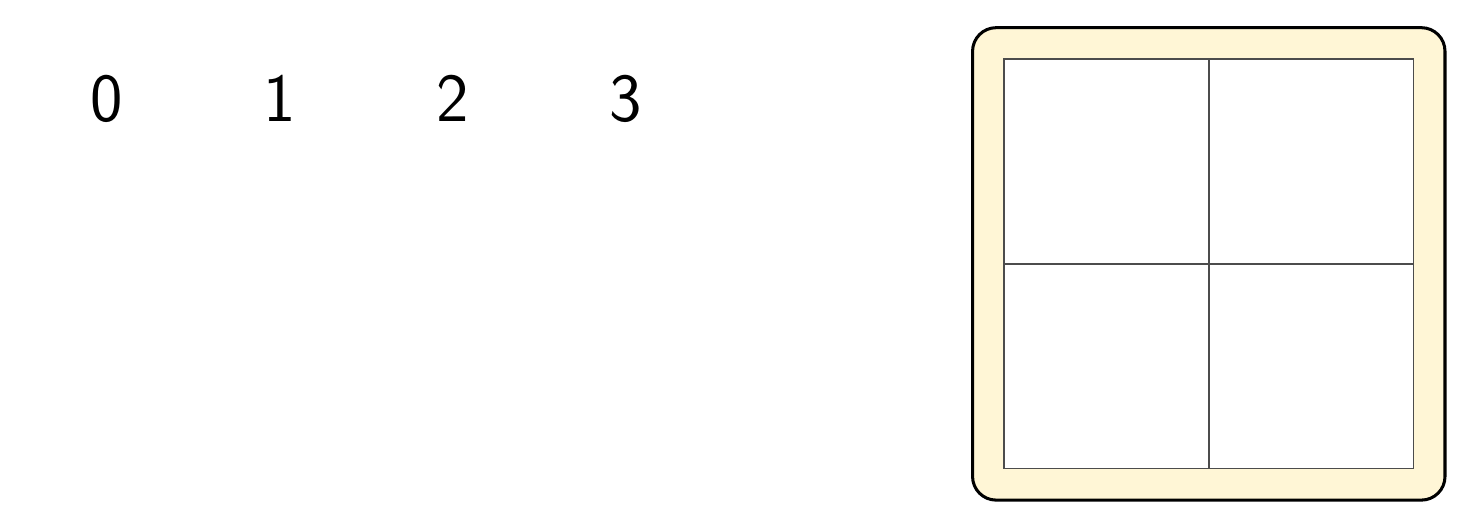
\begin{tikzpicture}[x=1mm,y=1mm]
\useasboundingbox (0,0) rectangle (180,-60);
\node[font=\Huge] at (10,-9) {0};
\node[font=\Huge] at (32,-9) {1};
\node[font=\Huge] at (54,-9) {2};
\node[font=\Huge] at (76,-9) {3};
\filldraw[fill=cardfill,draw=black,line width=1.1pt,rounded corners=3mm] (120,-60) rectangle (180,0);
\filldraw[fill=white,draw=black!70,line width=0.6pt] (124,-56) rectangle (150,-30);
\filldraw[fill=white,draw=black!70,line width=0.6pt] (124,-30) rectangle (150,-4);
\filldraw[fill=white,draw=black!70,line width=0.6pt] (150,-56) rectangle (176,-30);
\filldraw[fill=white,draw=black!70,line width=0.6pt] (150,-30) rectangle (176,-4);
\end{tikzpicture}\par
\vfill
\newpage
\prob{2}Behind the folder, one partner builds the square from one of these cards and takes away groups of~4. The other partner sees only the leftover and circles every card that could have made it. Then show the card.\par
\vspace{7mm}
{\centering 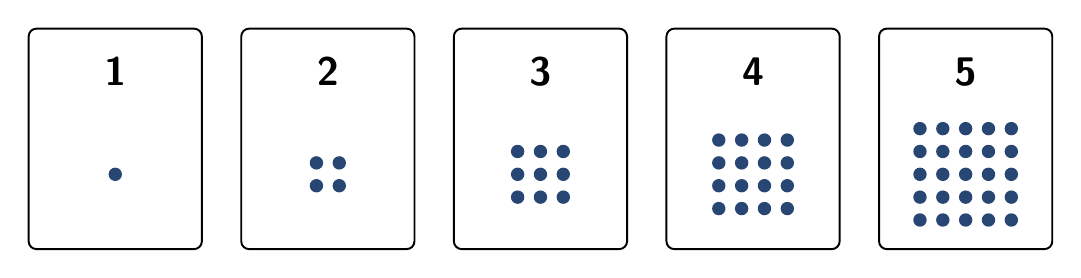
\begin{tikzpicture}[x=1mm,y=1mm]
\draw[line width=0.7pt,rounded corners=1mm] (0,0) rectangle (22,28);
\node[font=\Large\bfseries] at (11,22.5) {1};
\fill[tileline] (11,9.5) circle (0.85);
\draw[line width=0.7pt,rounded corners=1mm] (27,0) rectangle (49,28);
\node[font=\Large\bfseries] at (38,22.5) {2};
\fill[tileline] (36.55,8.05) circle (0.85);
\fill[tileline] (36.55,10.95) circle (0.85);
\fill[tileline] (39.45,8.05) circle (0.85);
\fill[tileline] (39.45,10.95) circle (0.85);
\draw[line width=0.7pt,rounded corners=1mm] (54,0) rectangle (76,28);
\node[font=\Large\bfseries] at (65,22.5) {3};
\fill[tileline] (62.1,6.6) circle (0.85);
\fill[tileline] (62.1,9.5) circle (0.85);
\fill[tileline] (62.1,12.4) circle (0.85);
\fill[tileline] (65,6.6) circle (0.85);
\fill[tileline] (65,9.5) circle (0.85);
\fill[tileline] (65,12.4) circle (0.85);
\fill[tileline] (67.9,6.6) circle (0.85);
\fill[tileline] (67.9,9.5) circle (0.85);
\fill[tileline] (67.9,12.4) circle (0.85);
\draw[line width=0.7pt,rounded corners=1mm] (81,0) rectangle (103,28);
\node[font=\Large\bfseries] at (92,22.5) {4};
\fill[tileline] (87.65,5.15) circle (0.85);
\fill[tileline] (87.65,8.05) circle (0.85);
\fill[tileline] (87.65,10.95) circle (0.85);
\fill[tileline] (87.65,13.85) circle (0.85);
\fill[tileline] (90.55,5.15) circle (0.85);
\fill[tileline] (90.55,8.05) circle (0.85);
\fill[tileline] (90.55,10.95) circle (0.85);
\fill[tileline] (90.55,13.85) circle (0.85);
\fill[tileline] (93.45,5.15) circle (0.85);
\fill[tileline] (93.45,8.05) circle (0.85);
\fill[tileline] (93.45,10.95) circle (0.85);
\fill[tileline] (93.45,13.85) circle (0.85);
\fill[tileline] (96.35,5.15) circle (0.85);
\fill[tileline] (96.35,8.05) circle (0.85);
\fill[tileline] (96.35,10.95) circle (0.85);
\fill[tileline] (96.35,13.85) circle (0.85);
\draw[line width=0.7pt,rounded corners=1mm] (108,0) rectangle (130,28);
\node[font=\Large\bfseries] at (119,22.5) {5};
\fill[tileline] (113.2,3.7) circle (0.85);
\fill[tileline] (113.2,6.6) circle (0.85);
\fill[tileline] (113.2,9.5) circle (0.85);
\fill[tileline] (113.2,12.4) circle (0.85);
\fill[tileline] (113.2,15.3) circle (0.85);
\fill[tileline] (116.1,3.7) circle (0.85);
\fill[tileline] (116.1,6.6) circle (0.85);
\fill[tileline] (116.1,9.5) circle (0.85);
\fill[tileline] (116.1,12.4) circle (0.85);
\fill[tileline] (116.1,15.3) circle (0.85);
\fill[tileline] (119,3.7) circle (0.85);
\fill[tileline] (119,6.6) circle (0.85);
\fill[tileline] (119,9.5) circle (0.85);
\fill[tileline] (119,12.4) circle (0.85);
\fill[tileline] (119,15.3) circle (0.85);
\fill[tileline] (121.9,3.7) circle (0.85);
\fill[tileline] (121.9,6.6) circle (0.85);
\fill[tileline] (121.9,9.5) circle (0.85);
\fill[tileline] (121.9,12.4) circle (0.85);
\fill[tileline] (121.9,15.3) circle (0.85);
\fill[tileline] (124.8,3.7) circle (0.85);
\fill[tileline] (124.8,6.6) circle (0.85);
\fill[tileline] (124.8,9.5) circle (0.85);
\fill[tileline] (124.8,12.4) circle (0.85);
\fill[tileline] (124.8,15.3) circle (0.85);
\end{tikzpicture}\par}
\vspace{10mm}
\noindent\hspace*{3mm}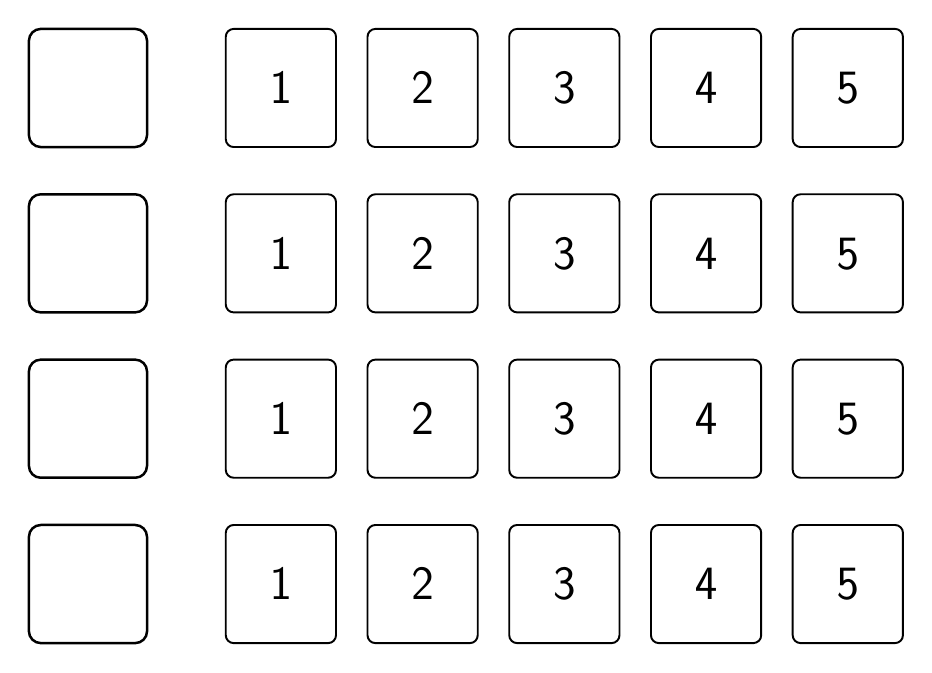
\begin{tikzpicture}[x=1mm,y=1mm]
\draw[wbox] (0,-15) rectangle (15,0);
\draw[line width=0.7pt,rounded corners=1mm] (25,-15) rectangle (39,0);
\node[font=\LARGE] at (32,-7.5) {1};
\draw[line width=0.7pt,rounded corners=1mm] (43,-15) rectangle (57,0);
\node[font=\LARGE] at (50,-7.5) {2};
\draw[line width=0.7pt,rounded corners=1mm] (61,-15) rectangle (75,0);
\node[font=\LARGE] at (68,-7.5) {3};
\draw[line width=0.7pt,rounded corners=1mm] (79,-15) rectangle (93,0);
\node[font=\LARGE] at (86,-7.5) {4};
\draw[line width=0.7pt,rounded corners=1mm] (97,-15) rectangle (111,0);
\node[font=\LARGE] at (104,-7.5) {5};
\draw[wbox] (0,-36) rectangle (15,-21);
\draw[line width=0.7pt,rounded corners=1mm] (25,-36) rectangle (39,-21);
\node[font=\LARGE] at (32,-28.5) {1};
\draw[line width=0.7pt,rounded corners=1mm] (43,-36) rectangle (57,-21);
\node[font=\LARGE] at (50,-28.5) {2};
\draw[line width=0.7pt,rounded corners=1mm] (61,-36) rectangle (75,-21);
\node[font=\LARGE] at (68,-28.5) {3};
\draw[line width=0.7pt,rounded corners=1mm] (79,-36) rectangle (93,-21);
\node[font=\LARGE] at (86,-28.5) {4};
\draw[line width=0.7pt,rounded corners=1mm] (97,-36) rectangle (111,-21);
\node[font=\LARGE] at (104,-28.5) {5};
\draw[wbox] (0,-57) rectangle (15,-42);
\draw[line width=0.7pt,rounded corners=1mm] (25,-57) rectangle (39,-42);
\node[font=\LARGE] at (32,-49.5) {1};
\draw[line width=0.7pt,rounded corners=1mm] (43,-57) rectangle (57,-42);
\node[font=\LARGE] at (50,-49.5) {2};
\draw[line width=0.7pt,rounded corners=1mm] (61,-57) rectangle (75,-42);
\node[font=\LARGE] at (68,-49.5) {3};
\draw[line width=0.7pt,rounded corners=1mm] (79,-57) rectangle (93,-42);
\node[font=\LARGE] at (86,-49.5) {4};
\draw[line width=0.7pt,rounded corners=1mm] (97,-57) rectangle (111,-42);
\node[font=\LARGE] at (104,-49.5) {5};
\draw[wbox] (0,-78) rectangle (15,-63);
\draw[line width=0.7pt,rounded corners=1mm] (25,-78) rectangle (39,-63);
\node[font=\LARGE] at (32,-70.5) {1};
\draw[line width=0.7pt,rounded corners=1mm] (43,-78) rectangle (57,-63);
\node[font=\LARGE] at (50,-70.5) {2};
\draw[line width=0.7pt,rounded corners=1mm] (61,-78) rectangle (75,-63);
\node[font=\LARGE] at (68,-70.5) {3};
\draw[line width=0.7pt,rounded corners=1mm] (79,-78) rectangle (93,-63);
\node[font=\LARGE] at (86,-70.5) {4};
\draw[line width=0.7pt,rounded corners=1mm] (97,-78) rectangle (111,-63);
\node[font=\LARGE] at (104,-70.5) {5};
\end{tikzpicture}\par
\vspace{8mm}
\noindent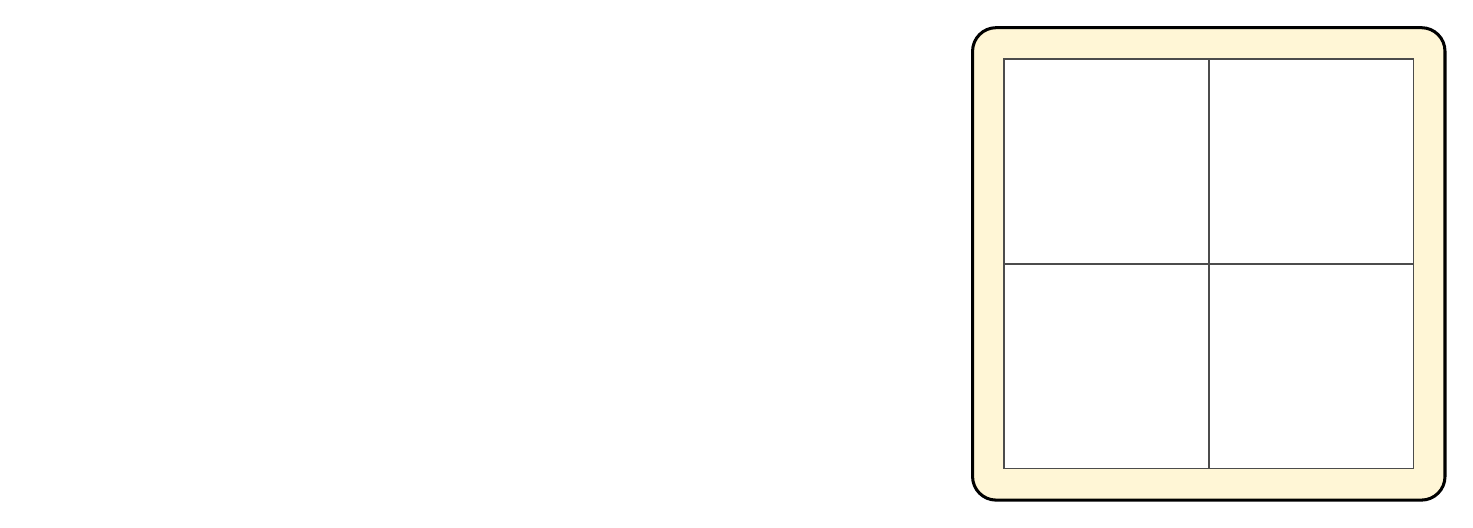
\begin{tikzpicture}[x=1mm,y=1mm]
\useasboundingbox (0,0) rectangle (180,-60);
\filldraw[fill=cardfill,draw=black,line width=1.1pt,rounded corners=3mm] (120,-60) rectangle (180,0);
\filldraw[fill=white,draw=black!70,line width=0.6pt] (124,-56) rectangle (150,-30);
\filldraw[fill=white,draw=black!70,line width=0.6pt] (124,-30) rectangle (150,-4);
\filldraw[fill=white,draw=black!70,line width=0.6pt] (150,-56) rectangle (176,-30);
\filldraw[fill=white,draw=black!70,line width=0.6pt] (150,-30) rectangle (176,-4);
\end{tikzpicture}\par
\vfill
\newpage
\prob{3}Build each rectangle and take away groups of~4. Can a rectangle leave 2~or~3?\par
\vspace{10mm}
{\centering 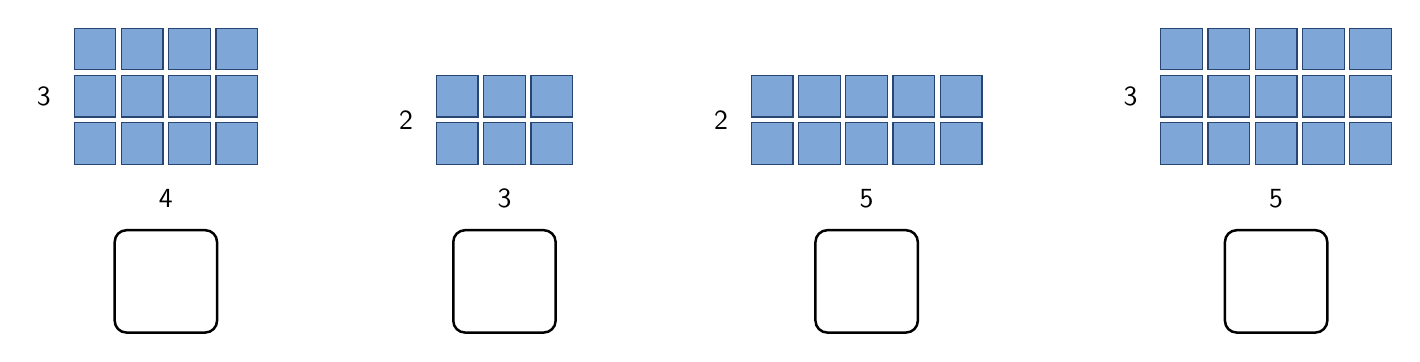
\begin{tikzpicture}[x=1mm,y=1mm]
\filldraw[tile] (0.36,0.36) rectangle (5.64,5.64);
\filldraw[tile] (0.36,6.36) rectangle (5.64,11.64);
\filldraw[tile] (0.36,12.36) rectangle (5.64,17.64);
\filldraw[tile] (6.36,0.36) rectangle (11.64,5.64);
\filldraw[tile] (6.36,6.36) rectangle (11.64,11.64);
\filldraw[tile] (6.36,12.36) rectangle (11.64,17.64);
\filldraw[tile] (12.36,0.36) rectangle (17.64,5.64);
\filldraw[tile] (12.36,6.36) rectangle (17.64,11.64);
\filldraw[tile] (12.36,12.36) rectangle (17.64,17.64);
\filldraw[tile] (18.36,0.36) rectangle (23.64,5.64);
\filldraw[tile] (18.36,6.36) rectangle (23.64,11.64);
\filldraw[tile] (18.36,12.36) rectangle (23.64,17.64);
\node[lab] at (12,-4) {4};
\node[lab] at (-3.5,9) {3};
\draw[wbox] (5.5,-21) rectangle (18.5,-8);
\filldraw[tile] (46.36,0.36) rectangle (51.64,5.64);
\filldraw[tile] (46.36,6.36) rectangle (51.64,11.64);
\filldraw[tile] (52.36,0.36) rectangle (57.64,5.64);
\filldraw[tile] (52.36,6.36) rectangle (57.64,11.64);
\filldraw[tile] (58.36,0.36) rectangle (63.64,5.64);
\filldraw[tile] (58.36,6.36) rectangle (63.64,11.64);
\node[lab] at (55,-4) {3};
\node[lab] at (42.5,6) {2};
\draw[wbox] (48.5,-21) rectangle (61.5,-8);
\filldraw[tile] (86.36,0.36) rectangle (91.64,5.64);
\filldraw[tile] (86.36,6.36) rectangle (91.64,11.64);
\filldraw[tile] (92.36,0.36) rectangle (97.64,5.64);
\filldraw[tile] (92.36,6.36) rectangle (97.64,11.64);
\filldraw[tile] (98.36,0.36) rectangle (103.64,5.64);
\filldraw[tile] (98.36,6.36) rectangle (103.64,11.64);
\filldraw[tile] (104.36,0.36) rectangle (109.64,5.64);
\filldraw[tile] (104.36,6.36) rectangle (109.64,11.64);
\filldraw[tile] (110.36,0.36) rectangle (115.64,5.64);
\filldraw[tile] (110.36,6.36) rectangle (115.64,11.64);
\node[lab] at (101,-4) {5};
\node[lab] at (82.5,6) {2};
\draw[wbox] (94.5,-21) rectangle (107.5,-8);
\filldraw[tile] (138.36,0.36) rectangle (143.64,5.64);
\filldraw[tile] (138.36,6.36) rectangle (143.64,11.64);
\filldraw[tile] (138.36,12.36) rectangle (143.64,17.64);
\filldraw[tile] (144.36,0.36) rectangle (149.64,5.64);
\filldraw[tile] (144.36,6.36) rectangle (149.64,11.64);
\filldraw[tile] (144.36,12.36) rectangle (149.64,17.64);
\filldraw[tile] (150.36,0.36) rectangle (155.64,5.64);
\filldraw[tile] (150.36,6.36) rectangle (155.64,11.64);
\filldraw[tile] (150.36,12.36) rectangle (155.64,17.64);
\filldraw[tile] (156.36,0.36) rectangle (161.64,5.64);
\filldraw[tile] (156.36,6.36) rectangle (161.64,11.64);
\filldraw[tile] (156.36,12.36) rectangle (161.64,17.64);
\filldraw[tile] (162.36,0.36) rectangle (167.64,5.64);
\filldraw[tile] (162.36,6.36) rectangle (167.64,11.64);
\filldraw[tile] (162.36,12.36) rectangle (167.64,17.64);
\node[lab] at (153,-4) {5};
\node[lab] at (134.5,9) {3};
\draw[wbox] (146.5,-21) rectangle (159.5,-8);
\end{tikzpicture}\par}
\vspace{10mm}
\noindent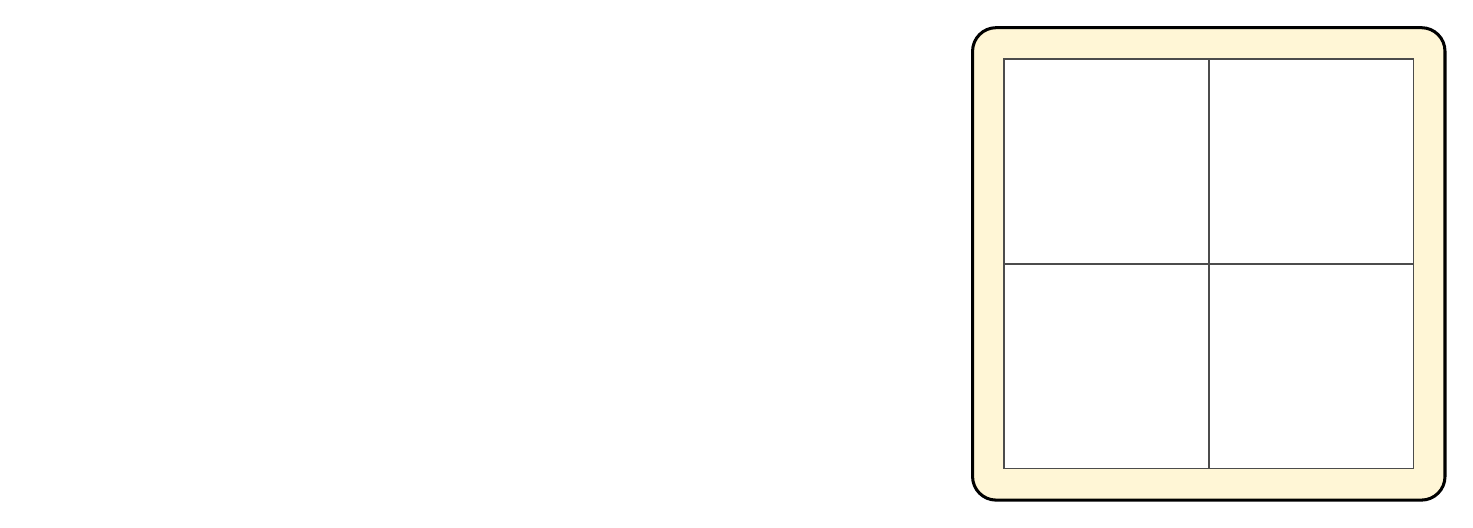
\begin{tikzpicture}[x=1mm,y=1mm]
\useasboundingbox (0,0) rectangle (180,-60);
\filldraw[fill=cardfill,draw=black,line width=1.1pt,rounded corners=3mm] (120,-60) rectangle (180,0);
\filldraw[fill=white,draw=black!70,line width=0.6pt] (124,-56) rectangle (150,-30);
\filldraw[fill=white,draw=black!70,line width=0.6pt] (124,-30) rectangle (150,-4);
\filldraw[fill=white,draw=black!70,line width=0.6pt] (150,-56) rectangle (176,-30);
\filldraw[fill=white,draw=black!70,line width=0.6pt] (150,-30) rectangle (176,-4);
\end{tikzpicture}\par
\vfill
\newpage
\prob{4}Build each square and take away groups of~3. Circle every number a square can leave.\par
\vspace{10mm}
{\centering 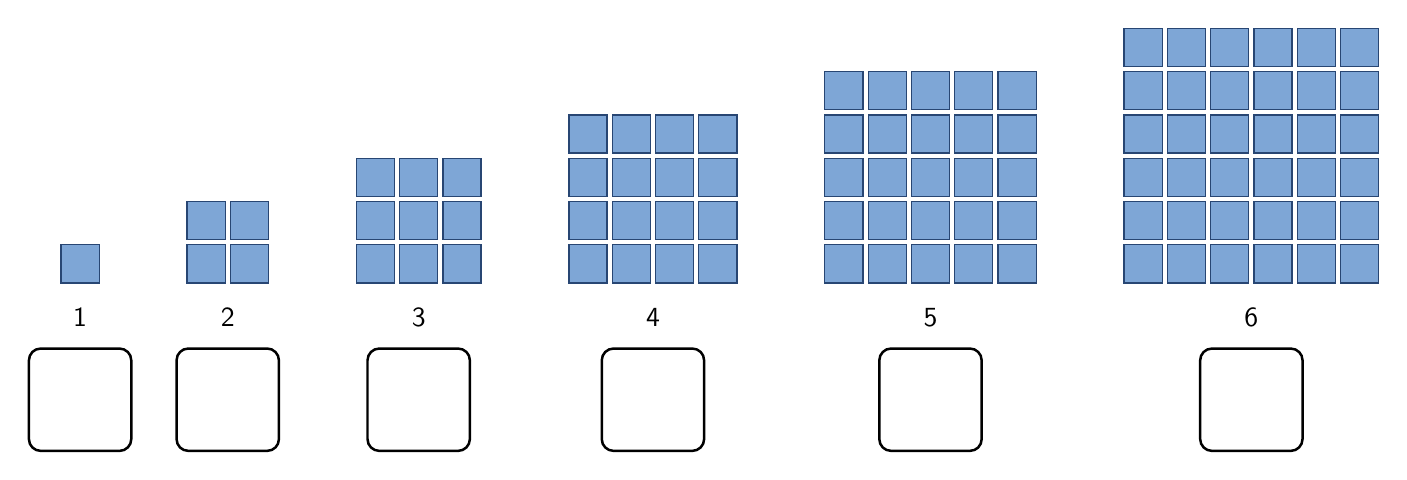
\begin{tikzpicture}[x=1mm,y=1mm]
\filldraw[tile] (0.33,0.33) rectangle (5.17,5.17);
\node[lab] at (2.75,-4) {1};
\draw[wbox] (-3.75,-21) rectangle (9.25,-8);
\filldraw[tile] (16.33,0.33) rectangle (21.17,5.17);
\filldraw[tile] (16.33,5.83) rectangle (21.17,10.67);
\filldraw[tile] (21.83,0.33) rectangle (26.67,5.17);
\filldraw[tile] (21.83,5.83) rectangle (26.67,10.67);
\node[lab] at (21.5,-4) {2};
\draw[wbox] (15,-21) rectangle (28,-8);
\filldraw[tile] (37.83,0.33) rectangle (42.67,5.17);
\filldraw[tile] (37.83,5.83) rectangle (42.67,10.67);
\filldraw[tile] (37.83,11.33) rectangle (42.67,16.17);
\filldraw[tile] (43.33,0.33) rectangle (48.17,5.17);
\filldraw[tile] (43.33,5.83) rectangle (48.17,10.67);
\filldraw[tile] (43.33,11.33) rectangle (48.17,16.17);
\filldraw[tile] (48.83,0.33) rectangle (53.67,5.17);
\filldraw[tile] (48.83,5.83) rectangle (53.67,10.67);
\filldraw[tile] (48.83,11.33) rectangle (53.67,16.17);
\node[lab] at (45.75,-4) {3};
\draw[wbox] (39.25,-21) rectangle (52.25,-8);
\filldraw[tile] (64.83,0.33) rectangle (69.67,5.17);
\filldraw[tile] (64.83,5.83) rectangle (69.67,10.67);
\filldraw[tile] (64.83,11.33) rectangle (69.67,16.17);
\filldraw[tile] (64.83,16.83) rectangle (69.67,21.67);
\filldraw[tile] (70.33,0.33) rectangle (75.17,5.17);
\filldraw[tile] (70.33,5.83) rectangle (75.17,10.67);
\filldraw[tile] (70.33,11.33) rectangle (75.17,16.17);
\filldraw[tile] (70.33,16.83) rectangle (75.17,21.67);
\filldraw[tile] (75.83,0.33) rectangle (80.67,5.17);
\filldraw[tile] (75.83,5.83) rectangle (80.67,10.67);
\filldraw[tile] (75.83,11.33) rectangle (80.67,16.17);
\filldraw[tile] (75.83,16.83) rectangle (80.67,21.67);
\filldraw[tile] (81.33,0.33) rectangle (86.17,5.17);
\filldraw[tile] (81.33,5.83) rectangle (86.17,10.67);
\filldraw[tile] (81.33,11.33) rectangle (86.17,16.17);
\filldraw[tile] (81.33,16.83) rectangle (86.17,21.67);
\node[lab] at (75.5,-4) {4};
\draw[wbox] (69,-21) rectangle (82,-8);
\filldraw[tile] (97.33,0.33) rectangle (102.17,5.17);
\filldraw[tile] (97.33,5.83) rectangle (102.17,10.67);
\filldraw[tile] (97.33,11.33) rectangle (102.17,16.17);
\filldraw[tile] (97.33,16.83) rectangle (102.17,21.67);
\filldraw[tile] (97.33,22.33) rectangle (102.17,27.17);
\filldraw[tile] (102.83,0.33) rectangle (107.67,5.17);
\filldraw[tile] (102.83,5.83) rectangle (107.67,10.67);
\filldraw[tile] (102.83,11.33) rectangle (107.67,16.17);
\filldraw[tile] (102.83,16.83) rectangle (107.67,21.67);
\filldraw[tile] (102.83,22.33) rectangle (107.67,27.17);
\filldraw[tile] (108.33,0.33) rectangle (113.17,5.17);
\filldraw[tile] (108.33,5.83) rectangle (113.17,10.67);
\filldraw[tile] (108.33,11.33) rectangle (113.17,16.17);
\filldraw[tile] (108.33,16.83) rectangle (113.17,21.67);
\filldraw[tile] (108.33,22.33) rectangle (113.17,27.17);
\filldraw[tile] (113.83,0.33) rectangle (118.67,5.17);
\filldraw[tile] (113.83,5.83) rectangle (118.67,10.67);
\filldraw[tile] (113.83,11.33) rectangle (118.67,16.17);
\filldraw[tile] (113.83,16.83) rectangle (118.67,21.67);
\filldraw[tile] (113.83,22.33) rectangle (118.67,27.17);
\filldraw[tile] (119.33,0.33) rectangle (124.17,5.17);
\filldraw[tile] (119.33,5.83) rectangle (124.17,10.67);
\filldraw[tile] (119.33,11.33) rectangle (124.17,16.17);
\filldraw[tile] (119.33,16.83) rectangle (124.17,21.67);
\filldraw[tile] (119.33,22.33) rectangle (124.17,27.17);
\node[lab] at (110.75,-4) {5};
\draw[wbox] (104.25,-21) rectangle (117.25,-8);
\filldraw[tile] (135.33,0.33) rectangle (140.17,5.17);
\filldraw[tile] (135.33,5.83) rectangle (140.17,10.67);
\filldraw[tile] (135.33,11.33) rectangle (140.17,16.17);
\filldraw[tile] (135.33,16.83) rectangle (140.17,21.67);
\filldraw[tile] (135.33,22.33) rectangle (140.17,27.17);
\filldraw[tile] (135.33,27.83) rectangle (140.17,32.67);
\filldraw[tile] (140.83,0.33) rectangle (145.67,5.17);
\filldraw[tile] (140.83,5.83) rectangle (145.67,10.67);
\filldraw[tile] (140.83,11.33) rectangle (145.67,16.17);
\filldraw[tile] (140.83,16.83) rectangle (145.67,21.67);
\filldraw[tile] (140.83,22.33) rectangle (145.67,27.17);
\filldraw[tile] (140.83,27.83) rectangle (145.67,32.67);
\filldraw[tile] (146.33,0.33) rectangle (151.17,5.17);
\filldraw[tile] (146.33,5.83) rectangle (151.17,10.67);
\filldraw[tile] (146.33,11.33) rectangle (151.17,16.17);
\filldraw[tile] (146.33,16.83) rectangle (151.17,21.67);
\filldraw[tile] (146.33,22.33) rectangle (151.17,27.17);
\filldraw[tile] (146.33,27.83) rectangle (151.17,32.67);
\filldraw[tile] (151.83,0.33) rectangle (156.67,5.17);
\filldraw[tile] (151.83,5.83) rectangle (156.67,10.67);
\filldraw[tile] (151.83,11.33) rectangle (156.67,16.17);
\filldraw[tile] (151.83,16.83) rectangle (156.67,21.67);
\filldraw[tile] (151.83,22.33) rectangle (156.67,27.17);
\filldraw[tile] (151.83,27.83) rectangle (156.67,32.67);
\filldraw[tile] (157.33,0.33) rectangle (162.17,5.17);
\filldraw[tile] (157.33,5.83) rectangle (162.17,10.67);
\filldraw[tile] (157.33,11.33) rectangle (162.17,16.17);
\filldraw[tile] (157.33,16.83) rectangle (162.17,21.67);
\filldraw[tile] (157.33,22.33) rectangle (162.17,27.17);
\filldraw[tile] (157.33,27.83) rectangle (162.17,32.67);
\filldraw[tile] (162.83,0.33) rectangle (167.67,5.17);
\filldraw[tile] (162.83,5.83) rectangle (167.67,10.67);
\filldraw[tile] (162.83,11.33) rectangle (167.67,16.17);
\filldraw[tile] (162.83,16.83) rectangle (167.67,21.67);
\filldraw[tile] (162.83,22.33) rectangle (167.67,27.17);
\filldraw[tile] (162.83,27.83) rectangle (167.67,32.67);
\node[lab] at (151.5,-4) {6};
\draw[wbox] (145,-21) rectangle (158,-8);
\end{tikzpicture}\par}
\vspace{10mm}
\noindent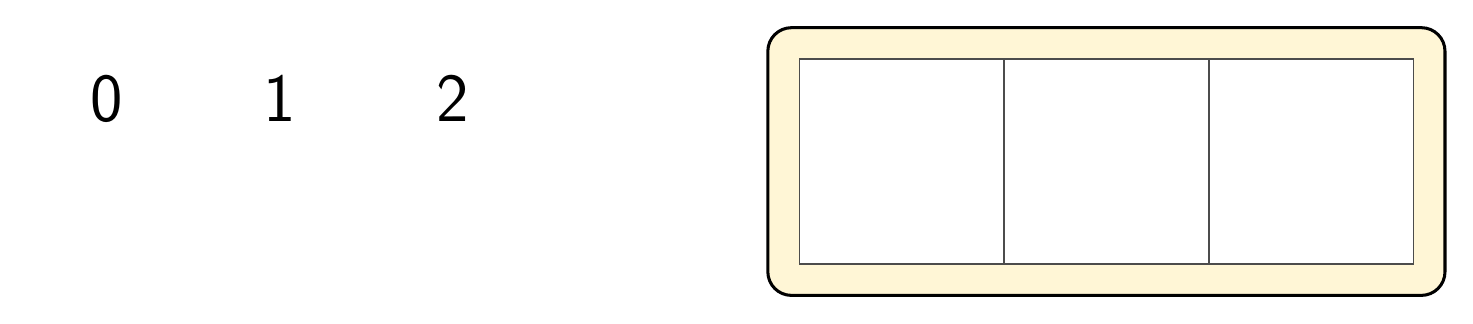
\begin{tikzpicture}[x=1mm,y=1mm]
\useasboundingbox (0,0) rectangle (180,-34);
\node[font=\Huge] at (10,-9) {0};
\node[font=\Huge] at (32,-9) {1};
\node[font=\Huge] at (54,-9) {2};
\filldraw[fill=cardfill,draw=black,line width=1.1pt,rounded corners=3mm] (94,-34) rectangle (180,0);
\filldraw[fill=white,draw=black!70,line width=0.6pt] (98,-30) rectangle (124,-4);
\filldraw[fill=white,draw=black!70,line width=0.6pt] (124,-30) rectangle (150,-4);
\filldraw[fill=white,draw=black!70,line width=0.6pt] (150,-30) rectangle (176,-4);
\end{tikzpicture}\par
\vfill
\newpage
\prob{5}Build each square and take away groups of~6. Circle every number a square can leave.\par
\vspace{10mm}
{\centering 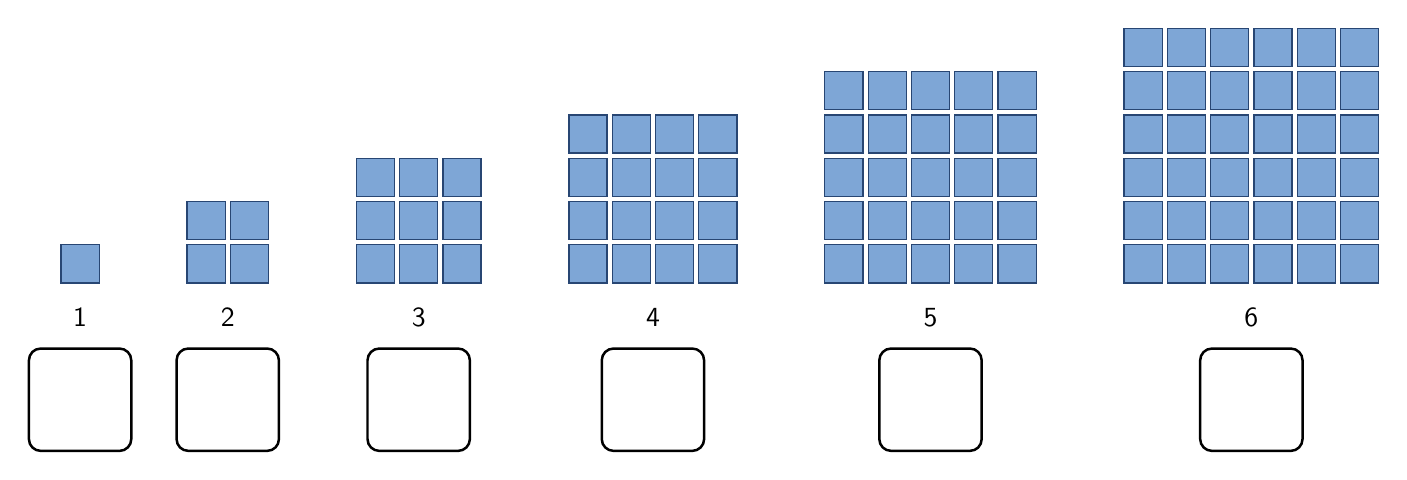
\begin{tikzpicture}[x=1mm,y=1mm]
\filldraw[tile] (0.33,0.33) rectangle (5.17,5.17);
\node[lab] at (2.75,-4) {1};
\draw[wbox] (-3.75,-21) rectangle (9.25,-8);
\filldraw[tile] (16.33,0.33) rectangle (21.17,5.17);
\filldraw[tile] (16.33,5.83) rectangle (21.17,10.67);
\filldraw[tile] (21.83,0.33) rectangle (26.67,5.17);
\filldraw[tile] (21.83,5.83) rectangle (26.67,10.67);
\node[lab] at (21.5,-4) {2};
\draw[wbox] (15,-21) rectangle (28,-8);
\filldraw[tile] (37.83,0.33) rectangle (42.67,5.17);
\filldraw[tile] (37.83,5.83) rectangle (42.67,10.67);
\filldraw[tile] (37.83,11.33) rectangle (42.67,16.17);
\filldraw[tile] (43.33,0.33) rectangle (48.17,5.17);
\filldraw[tile] (43.33,5.83) rectangle (48.17,10.67);
\filldraw[tile] (43.33,11.33) rectangle (48.17,16.17);
\filldraw[tile] (48.83,0.33) rectangle (53.67,5.17);
\filldraw[tile] (48.83,5.83) rectangle (53.67,10.67);
\filldraw[tile] (48.83,11.33) rectangle (53.67,16.17);
\node[lab] at (45.75,-4) {3};
\draw[wbox] (39.25,-21) rectangle (52.25,-8);
\filldraw[tile] (64.83,0.33) rectangle (69.67,5.17);
\filldraw[tile] (64.83,5.83) rectangle (69.67,10.67);
\filldraw[tile] (64.83,11.33) rectangle (69.67,16.17);
\filldraw[tile] (64.83,16.83) rectangle (69.67,21.67);
\filldraw[tile] (70.33,0.33) rectangle (75.17,5.17);
\filldraw[tile] (70.33,5.83) rectangle (75.17,10.67);
\filldraw[tile] (70.33,11.33) rectangle (75.17,16.17);
\filldraw[tile] (70.33,16.83) rectangle (75.17,21.67);
\filldraw[tile] (75.83,0.33) rectangle (80.67,5.17);
\filldraw[tile] (75.83,5.83) rectangle (80.67,10.67);
\filldraw[tile] (75.83,11.33) rectangle (80.67,16.17);
\filldraw[tile] (75.83,16.83) rectangle (80.67,21.67);
\filldraw[tile] (81.33,0.33) rectangle (86.17,5.17);
\filldraw[tile] (81.33,5.83) rectangle (86.17,10.67);
\filldraw[tile] (81.33,11.33) rectangle (86.17,16.17);
\filldraw[tile] (81.33,16.83) rectangle (86.17,21.67);
\node[lab] at (75.5,-4) {4};
\draw[wbox] (69,-21) rectangle (82,-8);
\filldraw[tile] (97.33,0.33) rectangle (102.17,5.17);
\filldraw[tile] (97.33,5.83) rectangle (102.17,10.67);
\filldraw[tile] (97.33,11.33) rectangle (102.17,16.17);
\filldraw[tile] (97.33,16.83) rectangle (102.17,21.67);
\filldraw[tile] (97.33,22.33) rectangle (102.17,27.17);
\filldraw[tile] (102.83,0.33) rectangle (107.67,5.17);
\filldraw[tile] (102.83,5.83) rectangle (107.67,10.67);
\filldraw[tile] (102.83,11.33) rectangle (107.67,16.17);
\filldraw[tile] (102.83,16.83) rectangle (107.67,21.67);
\filldraw[tile] (102.83,22.33) rectangle (107.67,27.17);
\filldraw[tile] (108.33,0.33) rectangle (113.17,5.17);
\filldraw[tile] (108.33,5.83) rectangle (113.17,10.67);
\filldraw[tile] (108.33,11.33) rectangle (113.17,16.17);
\filldraw[tile] (108.33,16.83) rectangle (113.17,21.67);
\filldraw[tile] (108.33,22.33) rectangle (113.17,27.17);
\filldraw[tile] (113.83,0.33) rectangle (118.67,5.17);
\filldraw[tile] (113.83,5.83) rectangle (118.67,10.67);
\filldraw[tile] (113.83,11.33) rectangle (118.67,16.17);
\filldraw[tile] (113.83,16.83) rectangle (118.67,21.67);
\filldraw[tile] (113.83,22.33) rectangle (118.67,27.17);
\filldraw[tile] (119.33,0.33) rectangle (124.17,5.17);
\filldraw[tile] (119.33,5.83) rectangle (124.17,10.67);
\filldraw[tile] (119.33,11.33) rectangle (124.17,16.17);
\filldraw[tile] (119.33,16.83) rectangle (124.17,21.67);
\filldraw[tile] (119.33,22.33) rectangle (124.17,27.17);
\node[lab] at (110.75,-4) {5};
\draw[wbox] (104.25,-21) rectangle (117.25,-8);
\filldraw[tile] (135.33,0.33) rectangle (140.17,5.17);
\filldraw[tile] (135.33,5.83) rectangle (140.17,10.67);
\filldraw[tile] (135.33,11.33) rectangle (140.17,16.17);
\filldraw[tile] (135.33,16.83) rectangle (140.17,21.67);
\filldraw[tile] (135.33,22.33) rectangle (140.17,27.17);
\filldraw[tile] (135.33,27.83) rectangle (140.17,32.67);
\filldraw[tile] (140.83,0.33) rectangle (145.67,5.17);
\filldraw[tile] (140.83,5.83) rectangle (145.67,10.67);
\filldraw[tile] (140.83,11.33) rectangle (145.67,16.17);
\filldraw[tile] (140.83,16.83) rectangle (145.67,21.67);
\filldraw[tile] (140.83,22.33) rectangle (145.67,27.17);
\filldraw[tile] (140.83,27.83) rectangle (145.67,32.67);
\filldraw[tile] (146.33,0.33) rectangle (151.17,5.17);
\filldraw[tile] (146.33,5.83) rectangle (151.17,10.67);
\filldraw[tile] (146.33,11.33) rectangle (151.17,16.17);
\filldraw[tile] (146.33,16.83) rectangle (151.17,21.67);
\filldraw[tile] (146.33,22.33) rectangle (151.17,27.17);
\filldraw[tile] (146.33,27.83) rectangle (151.17,32.67);
\filldraw[tile] (151.83,0.33) rectangle (156.67,5.17);
\filldraw[tile] (151.83,5.83) rectangle (156.67,10.67);
\filldraw[tile] (151.83,11.33) rectangle (156.67,16.17);
\filldraw[tile] (151.83,16.83) rectangle (156.67,21.67);
\filldraw[tile] (151.83,22.33) rectangle (156.67,27.17);
\filldraw[tile] (151.83,27.83) rectangle (156.67,32.67);
\filldraw[tile] (157.33,0.33) rectangle (162.17,5.17);
\filldraw[tile] (157.33,5.83) rectangle (162.17,10.67);
\filldraw[tile] (157.33,11.33) rectangle (162.17,16.17);
\filldraw[tile] (157.33,16.83) rectangle (162.17,21.67);
\filldraw[tile] (157.33,22.33) rectangle (162.17,27.17);
\filldraw[tile] (157.33,27.83) rectangle (162.17,32.67);
\filldraw[tile] (162.83,0.33) rectangle (167.67,5.17);
\filldraw[tile] (162.83,5.83) rectangle (167.67,10.67);
\filldraw[tile] (162.83,11.33) rectangle (167.67,16.17);
\filldraw[tile] (162.83,16.83) rectangle (167.67,21.67);
\filldraw[tile] (162.83,22.33) rectangle (167.67,27.17);
\filldraw[tile] (162.83,27.83) rectangle (167.67,32.67);
\node[lab] at (151.5,-4) {6};
\draw[wbox] (145,-21) rectangle (158,-8);
\end{tikzpicture}\par}
\vspace{10mm}
\noindent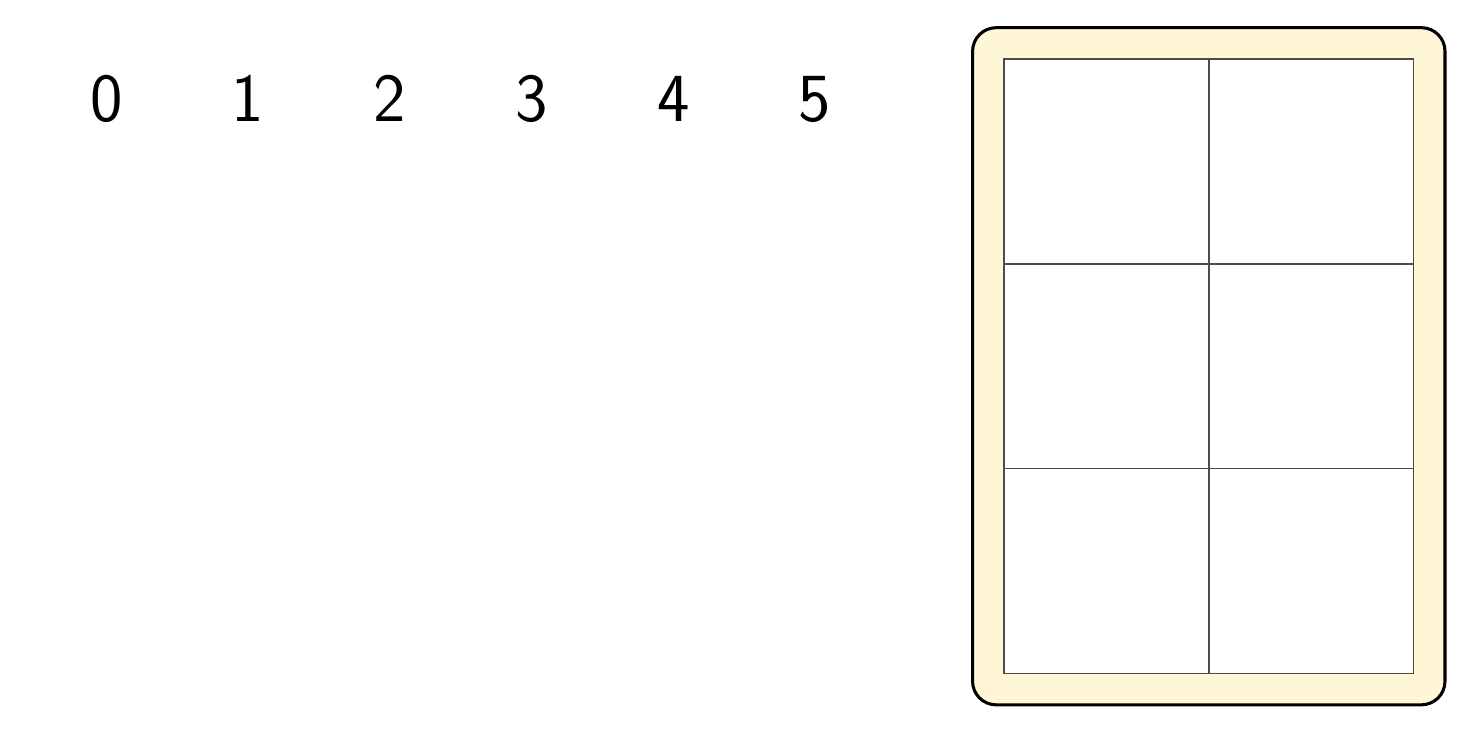
\begin{tikzpicture}[x=1mm,y=1mm]
\useasboundingbox (0,0) rectangle (180,-86);
\node[font=\Huge] at (10,-9) {0};
\node[font=\Huge] at (28,-9) {1};
\node[font=\Huge] at (46,-9) {2};
\node[font=\Huge] at (64,-9) {3};
\node[font=\Huge] at (82,-9) {4};
\node[font=\Huge] at (100,-9) {5};
\filldraw[fill=cardfill,draw=black,line width=1.1pt,rounded corners=3mm] (120,-86) rectangle (180,0);
\filldraw[fill=white,draw=black!70,line width=0.6pt] (124,-82) rectangle (150,-56);
\filldraw[fill=white,draw=black!70,line width=0.6pt] (124,-56) rectangle (150,-30);
\filldraw[fill=white,draw=black!70,line width=0.6pt] (124,-30) rectangle (150,-4);
\filldraw[fill=white,draw=black!70,line width=0.6pt] (150,-82) rectangle (176,-56);
\filldraw[fill=white,draw=black!70,line width=0.6pt] (150,-56) rectangle (176,-30);
\filldraw[fill=white,draw=black!70,line width=0.6pt] (150,-30) rectangle (176,-4);
\end{tikzpicture}\par
\vfill
\newpage
\prob{6}Play Problem~2 again with these cards and groups of~6.\par
\vspace{7mm}
{\centering 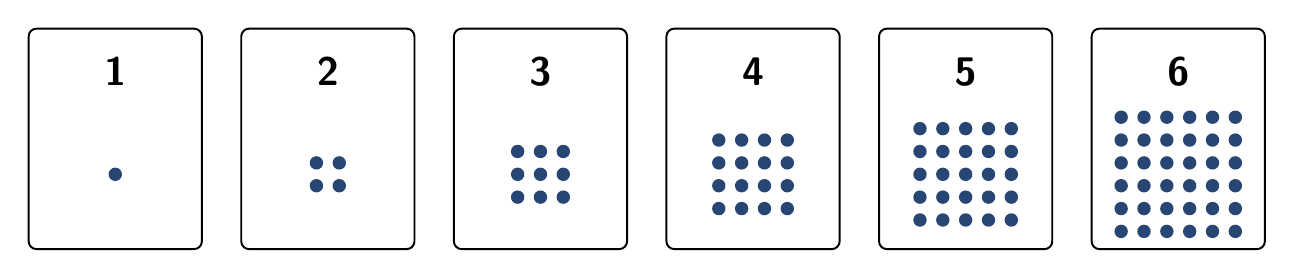
\begin{tikzpicture}[x=1mm,y=1mm]
\draw[line width=0.7pt,rounded corners=1mm] (0,0) rectangle (22,28);
\node[font=\Large\bfseries] at (11,22.5) {1};
\fill[tileline] (11,9.5) circle (0.85);
\draw[line width=0.7pt,rounded corners=1mm] (27,0) rectangle (49,28);
\node[font=\Large\bfseries] at (38,22.5) {2};
\fill[tileline] (36.55,8.05) circle (0.85);
\fill[tileline] (36.55,10.95) circle (0.85);
\fill[tileline] (39.45,8.05) circle (0.85);
\fill[tileline] (39.45,10.95) circle (0.85);
\draw[line width=0.7pt,rounded corners=1mm] (54,0) rectangle (76,28);
\node[font=\Large\bfseries] at (65,22.5) {3};
\fill[tileline] (62.1,6.6) circle (0.85);
\fill[tileline] (62.1,9.5) circle (0.85);
\fill[tileline] (62.1,12.4) circle (0.85);
\fill[tileline] (65,6.6) circle (0.85);
\fill[tileline] (65,9.5) circle (0.85);
\fill[tileline] (65,12.4) circle (0.85);
\fill[tileline] (67.9,6.6) circle (0.85);
\fill[tileline] (67.9,9.5) circle (0.85);
\fill[tileline] (67.9,12.4) circle (0.85);
\draw[line width=0.7pt,rounded corners=1mm] (81,0) rectangle (103,28);
\node[font=\Large\bfseries] at (92,22.5) {4};
\fill[tileline] (87.65,5.15) circle (0.85);
\fill[tileline] (87.65,8.05) circle (0.85);
\fill[tileline] (87.65,10.95) circle (0.85);
\fill[tileline] (87.65,13.85) circle (0.85);
\fill[tileline] (90.55,5.15) circle (0.85);
\fill[tileline] (90.55,8.05) circle (0.85);
\fill[tileline] (90.55,10.95) circle (0.85);
\fill[tileline] (90.55,13.85) circle (0.85);
\fill[tileline] (93.45,5.15) circle (0.85);
\fill[tileline] (93.45,8.05) circle (0.85);
\fill[tileline] (93.45,10.95) circle (0.85);
\fill[tileline] (93.45,13.85) circle (0.85);
\fill[tileline] (96.35,5.15) circle (0.85);
\fill[tileline] (96.35,8.05) circle (0.85);
\fill[tileline] (96.35,10.95) circle (0.85);
\fill[tileline] (96.35,13.85) circle (0.85);
\draw[line width=0.7pt,rounded corners=1mm] (108,0) rectangle (130,28);
\node[font=\Large\bfseries] at (119,22.5) {5};
\fill[tileline] (113.2,3.7) circle (0.85);
\fill[tileline] (113.2,6.6) circle (0.85);
\fill[tileline] (113.2,9.5) circle (0.85);
\fill[tileline] (113.2,12.4) circle (0.85);
\fill[tileline] (113.2,15.3) circle (0.85);
\fill[tileline] (116.1,3.7) circle (0.85);
\fill[tileline] (116.1,6.6) circle (0.85);
\fill[tileline] (116.1,9.5) circle (0.85);
\fill[tileline] (116.1,12.4) circle (0.85);
\fill[tileline] (116.1,15.3) circle (0.85);
\fill[tileline] (119,3.7) circle (0.85);
\fill[tileline] (119,6.6) circle (0.85);
\fill[tileline] (119,9.5) circle (0.85);
\fill[tileline] (119,12.4) circle (0.85);
\fill[tileline] (119,15.3) circle (0.85);
\fill[tileline] (121.9,3.7) circle (0.85);
\fill[tileline] (121.9,6.6) circle (0.85);
\fill[tileline] (121.9,9.5) circle (0.85);
\fill[tileline] (121.9,12.4) circle (0.85);
\fill[tileline] (121.9,15.3) circle (0.85);
\fill[tileline] (124.8,3.7) circle (0.85);
\fill[tileline] (124.8,6.6) circle (0.85);
\fill[tileline] (124.8,9.5) circle (0.85);
\fill[tileline] (124.8,12.4) circle (0.85);
\fill[tileline] (124.8,15.3) circle (0.85);
\draw[line width=0.7pt,rounded corners=1mm] (135,0) rectangle (157,28);
\node[font=\Large\bfseries] at (146,22.5) {6};
\fill[tileline] (138.75,2.25) circle (0.85);
\fill[tileline] (138.75,5.15) circle (0.85);
\fill[tileline] (138.75,8.05) circle (0.85);
\fill[tileline] (138.75,10.95) circle (0.85);
\fill[tileline] (138.75,13.85) circle (0.85);
\fill[tileline] (138.75,16.75) circle (0.85);
\fill[tileline] (141.65,2.25) circle (0.85);
\fill[tileline] (141.65,5.15) circle (0.85);
\fill[tileline] (141.65,8.05) circle (0.85);
\fill[tileline] (141.65,10.95) circle (0.85);
\fill[tileline] (141.65,13.85) circle (0.85);
\fill[tileline] (141.65,16.75) circle (0.85);
\fill[tileline] (144.55,2.25) circle (0.85);
\fill[tileline] (144.55,5.15) circle (0.85);
\fill[tileline] (144.55,8.05) circle (0.85);
\fill[tileline] (144.55,10.95) circle (0.85);
\fill[tileline] (144.55,13.85) circle (0.85);
\fill[tileline] (144.55,16.75) circle (0.85);
\fill[tileline] (147.45,2.25) circle (0.85);
\fill[tileline] (147.45,5.15) circle (0.85);
\fill[tileline] (147.45,8.05) circle (0.85);
\fill[tileline] (147.45,10.95) circle (0.85);
\fill[tileline] (147.45,13.85) circle (0.85);
\fill[tileline] (147.45,16.75) circle (0.85);
\fill[tileline] (150.35,2.25) circle (0.85);
\fill[tileline] (150.35,5.15) circle (0.85);
\fill[tileline] (150.35,8.05) circle (0.85);
\fill[tileline] (150.35,10.95) circle (0.85);
\fill[tileline] (150.35,13.85) circle (0.85);
\fill[tileline] (150.35,16.75) circle (0.85);
\fill[tileline] (153.25,2.25) circle (0.85);
\fill[tileline] (153.25,5.15) circle (0.85);
\fill[tileline] (153.25,8.05) circle (0.85);
\fill[tileline] (153.25,10.95) circle (0.85);
\fill[tileline] (153.25,13.85) circle (0.85);
\fill[tileline] (153.25,16.75) circle (0.85);
\end{tikzpicture}\par}
\vspace{10mm}
\noindent\hspace*{3mm}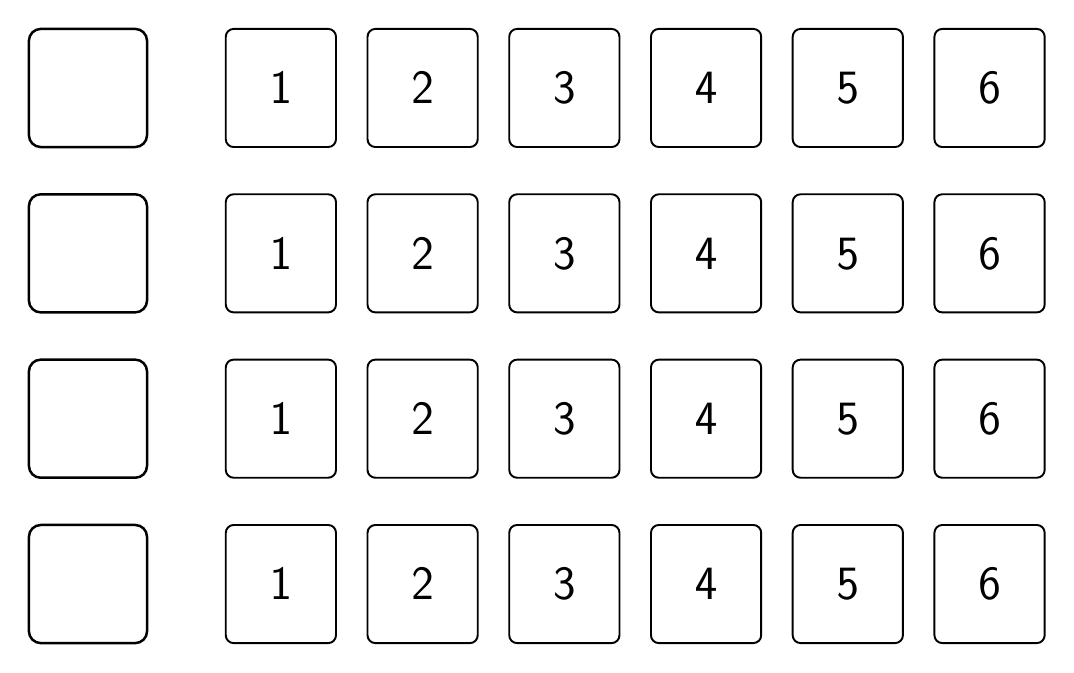
\begin{tikzpicture}[x=1mm,y=1mm]
\draw[wbox] (0,-15) rectangle (15,0);
\draw[line width=0.7pt,rounded corners=1mm] (25,-15) rectangle (39,0);
\node[font=\LARGE] at (32,-7.5) {1};
\draw[line width=0.7pt,rounded corners=1mm] (43,-15) rectangle (57,0);
\node[font=\LARGE] at (50,-7.5) {2};
\draw[line width=0.7pt,rounded corners=1mm] (61,-15) rectangle (75,0);
\node[font=\LARGE] at (68,-7.5) {3};
\draw[line width=0.7pt,rounded corners=1mm] (79,-15) rectangle (93,0);
\node[font=\LARGE] at (86,-7.5) {4};
\draw[line width=0.7pt,rounded corners=1mm] (97,-15) rectangle (111,0);
\node[font=\LARGE] at (104,-7.5) {5};
\draw[line width=0.7pt,rounded corners=1mm] (115,-15) rectangle (129,0);
\node[font=\LARGE] at (122,-7.5) {6};
\draw[wbox] (0,-36) rectangle (15,-21);
\draw[line width=0.7pt,rounded corners=1mm] (25,-36) rectangle (39,-21);
\node[font=\LARGE] at (32,-28.5) {1};
\draw[line width=0.7pt,rounded corners=1mm] (43,-36) rectangle (57,-21);
\node[font=\LARGE] at (50,-28.5) {2};
\draw[line width=0.7pt,rounded corners=1mm] (61,-36) rectangle (75,-21);
\node[font=\LARGE] at (68,-28.5) {3};
\draw[line width=0.7pt,rounded corners=1mm] (79,-36) rectangle (93,-21);
\node[font=\LARGE] at (86,-28.5) {4};
\draw[line width=0.7pt,rounded corners=1mm] (97,-36) rectangle (111,-21);
\node[font=\LARGE] at (104,-28.5) {5};
\draw[line width=0.7pt,rounded corners=1mm] (115,-36) rectangle (129,-21);
\node[font=\LARGE] at (122,-28.5) {6};
\draw[wbox] (0,-57) rectangle (15,-42);
\draw[line width=0.7pt,rounded corners=1mm] (25,-57) rectangle (39,-42);
\node[font=\LARGE] at (32,-49.5) {1};
\draw[line width=0.7pt,rounded corners=1mm] (43,-57) rectangle (57,-42);
\node[font=\LARGE] at (50,-49.5) {2};
\draw[line width=0.7pt,rounded corners=1mm] (61,-57) rectangle (75,-42);
\node[font=\LARGE] at (68,-49.5) {3};
\draw[line width=0.7pt,rounded corners=1mm] (79,-57) rectangle (93,-42);
\node[font=\LARGE] at (86,-49.5) {4};
\draw[line width=0.7pt,rounded corners=1mm] (97,-57) rectangle (111,-42);
\node[font=\LARGE] at (104,-49.5) {5};
\draw[line width=0.7pt,rounded corners=1mm] (115,-57) rectangle (129,-42);
\node[font=\LARGE] at (122,-49.5) {6};
\draw[wbox] (0,-78) rectangle (15,-63);
\draw[line width=0.7pt,rounded corners=1mm] (25,-78) rectangle (39,-63);
\node[font=\LARGE] at (32,-70.5) {1};
\draw[line width=0.7pt,rounded corners=1mm] (43,-78) rectangle (57,-63);
\node[font=\LARGE] at (50,-70.5) {2};
\draw[line width=0.7pt,rounded corners=1mm] (61,-78) rectangle (75,-63);
\node[font=\LARGE] at (68,-70.5) {3};
\draw[line width=0.7pt,rounded corners=1mm] (79,-78) rectangle (93,-63);
\node[font=\LARGE] at (86,-70.5) {4};
\draw[line width=0.7pt,rounded corners=1mm] (97,-78) rectangle (111,-63);
\node[font=\LARGE] at (104,-70.5) {5};
\draw[line width=0.7pt,rounded corners=1mm] (115,-78) rectangle (129,-63);
\node[font=\LARGE] at (122,-70.5) {6};
\end{tikzpicture}\par
\vspace{8mm}
\noindent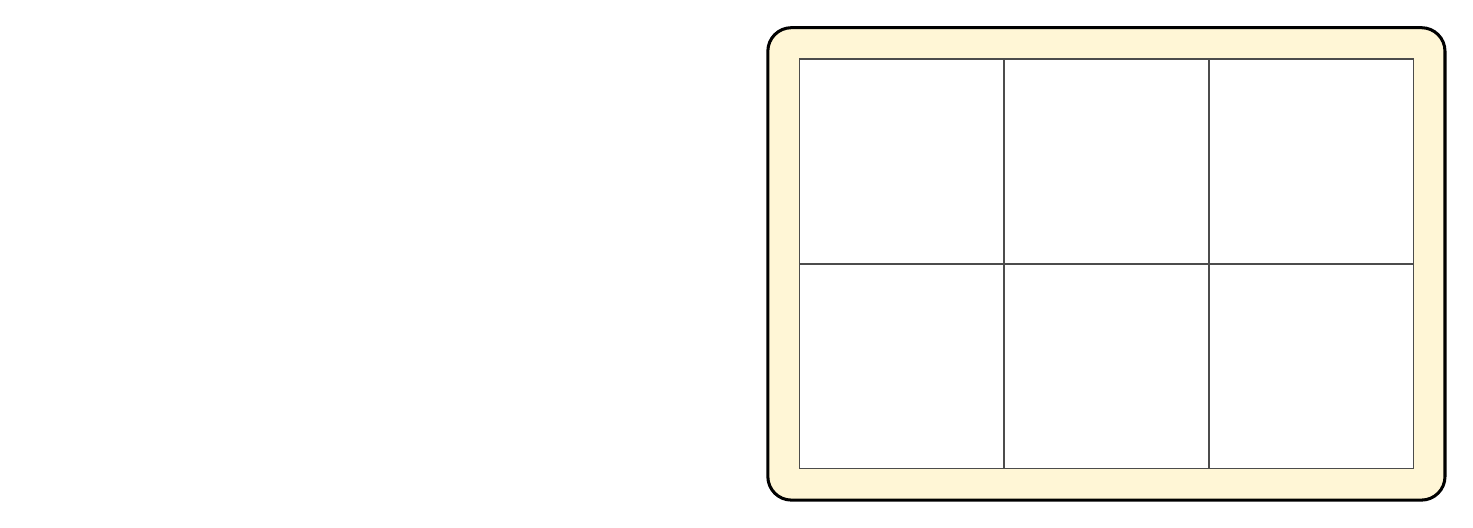
\begin{tikzpicture}[x=1mm,y=1mm]
\useasboundingbox (0,0) rectangle (180,-60);
\filldraw[fill=cardfill,draw=black,line width=1.1pt,rounded corners=3mm] (94,-60) rectangle (180,0);
\filldraw[fill=white,draw=black!70,line width=0.6pt] (98,-56) rectangle (124,-30);
\filldraw[fill=white,draw=black!70,line width=0.6pt] (98,-30) rectangle (124,-4);
\filldraw[fill=white,draw=black!70,line width=0.6pt] (124,-56) rectangle (150,-30);
\filldraw[fill=white,draw=black!70,line width=0.6pt] (124,-30) rectangle (150,-4);
\filldraw[fill=white,draw=black!70,line width=0.6pt] (150,-56) rectangle (176,-30);
\filldraw[fill=white,draw=black!70,line width=0.6pt] (150,-30) rectangle (176,-4);
\end{tikzpicture}\par
\vfill
\newpage
\prob{7}Build each square and take away groups of~2. Which squares leave~1?\par
\vspace{10mm}
{\centering 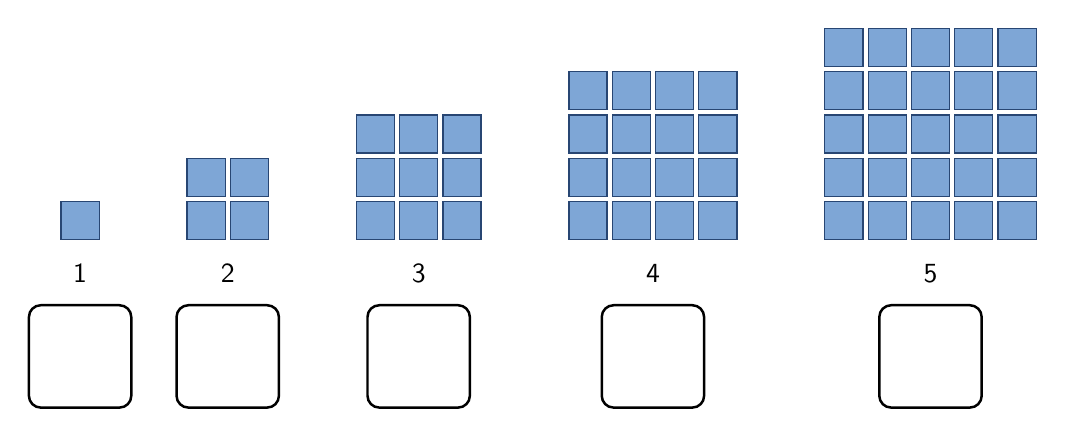
\begin{tikzpicture}[x=1mm,y=1mm]
\filldraw[tile] (0.33,0.33) rectangle (5.17,5.17);
\node[lab] at (2.75,-4) {1};
\draw[wbox] (-3.75,-21) rectangle (9.25,-8);
\filldraw[tile] (16.33,0.33) rectangle (21.17,5.17);
\filldraw[tile] (16.33,5.83) rectangle (21.17,10.67);
\filldraw[tile] (21.83,0.33) rectangle (26.67,5.17);
\filldraw[tile] (21.83,5.83) rectangle (26.67,10.67);
\node[lab] at (21.5,-4) {2};
\draw[wbox] (15,-21) rectangle (28,-8);
\filldraw[tile] (37.83,0.33) rectangle (42.67,5.17);
\filldraw[tile] (37.83,5.83) rectangle (42.67,10.67);
\filldraw[tile] (37.83,11.33) rectangle (42.67,16.17);
\filldraw[tile] (43.33,0.33) rectangle (48.17,5.17);
\filldraw[tile] (43.33,5.83) rectangle (48.17,10.67);
\filldraw[tile] (43.33,11.33) rectangle (48.17,16.17);
\filldraw[tile] (48.83,0.33) rectangle (53.67,5.17);
\filldraw[tile] (48.83,5.83) rectangle (53.67,10.67);
\filldraw[tile] (48.83,11.33) rectangle (53.67,16.17);
\node[lab] at (45.75,-4) {3};
\draw[wbox] (39.25,-21) rectangle (52.25,-8);
\filldraw[tile] (64.83,0.33) rectangle (69.67,5.17);
\filldraw[tile] (64.83,5.83) rectangle (69.67,10.67);
\filldraw[tile] (64.83,11.33) rectangle (69.67,16.17);
\filldraw[tile] (64.83,16.83) rectangle (69.67,21.67);
\filldraw[tile] (70.33,0.33) rectangle (75.17,5.17);
\filldraw[tile] (70.33,5.83) rectangle (75.17,10.67);
\filldraw[tile] (70.33,11.33) rectangle (75.17,16.17);
\filldraw[tile] (70.33,16.83) rectangle (75.17,21.67);
\filldraw[tile] (75.83,0.33) rectangle (80.67,5.17);
\filldraw[tile] (75.83,5.83) rectangle (80.67,10.67);
\filldraw[tile] (75.83,11.33) rectangle (80.67,16.17);
\filldraw[tile] (75.83,16.83) rectangle (80.67,21.67);
\filldraw[tile] (81.33,0.33) rectangle (86.17,5.17);
\filldraw[tile] (81.33,5.83) rectangle (86.17,10.67);
\filldraw[tile] (81.33,11.33) rectangle (86.17,16.17);
\filldraw[tile] (81.33,16.83) rectangle (86.17,21.67);
\node[lab] at (75.5,-4) {4};
\draw[wbox] (69,-21) rectangle (82,-8);
\filldraw[tile] (97.33,0.33) rectangle (102.17,5.17);
\filldraw[tile] (97.33,5.83) rectangle (102.17,10.67);
\filldraw[tile] (97.33,11.33) rectangle (102.17,16.17);
\filldraw[tile] (97.33,16.83) rectangle (102.17,21.67);
\filldraw[tile] (97.33,22.33) rectangle (102.17,27.17);
\filldraw[tile] (102.83,0.33) rectangle (107.67,5.17);
\filldraw[tile] (102.83,5.83) rectangle (107.67,10.67);
\filldraw[tile] (102.83,11.33) rectangle (107.67,16.17);
\filldraw[tile] (102.83,16.83) rectangle (107.67,21.67);
\filldraw[tile] (102.83,22.33) rectangle (107.67,27.17);
\filldraw[tile] (108.33,0.33) rectangle (113.17,5.17);
\filldraw[tile] (108.33,5.83) rectangle (113.17,10.67);
\filldraw[tile] (108.33,11.33) rectangle (113.17,16.17);
\filldraw[tile] (108.33,16.83) rectangle (113.17,21.67);
\filldraw[tile] (108.33,22.33) rectangle (113.17,27.17);
\filldraw[tile] (113.83,0.33) rectangle (118.67,5.17);
\filldraw[tile] (113.83,5.83) rectangle (118.67,10.67);
\filldraw[tile] (113.83,11.33) rectangle (118.67,16.17);
\filldraw[tile] (113.83,16.83) rectangle (118.67,21.67);
\filldraw[tile] (113.83,22.33) rectangle (118.67,27.17);
\filldraw[tile] (119.33,0.33) rectangle (124.17,5.17);
\filldraw[tile] (119.33,5.83) rectangle (124.17,10.67);
\filldraw[tile] (119.33,11.33) rectangle (124.17,16.17);
\filldraw[tile] (119.33,16.83) rectangle (124.17,21.67);
\filldraw[tile] (119.33,22.33) rectangle (124.17,27.17);
\node[lab] at (110.75,-4) {5};
\draw[wbox] (104.25,-21) rectangle (117.25,-8);
\end{tikzpicture}\par}
\vspace{10mm}
\noindent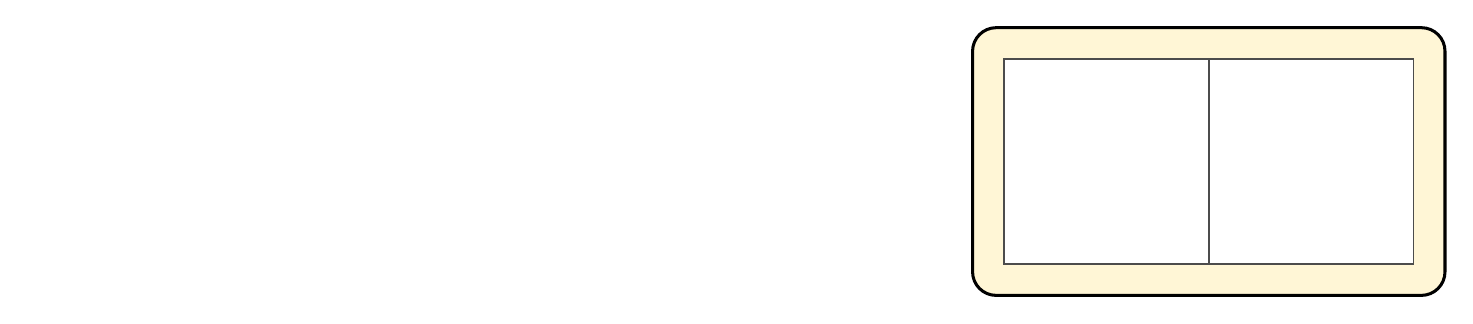
\begin{tikzpicture}[x=1mm,y=1mm]
\useasboundingbox (0,0) rectangle (180,-34);
\filldraw[fill=cardfill,draw=black,line width=1.1pt,rounded corners=3mm] (120,-34) rectangle (180,0);
\filldraw[fill=white,draw=black!70,line width=0.6pt] (124,-30) rectangle (150,-4);
\filldraw[fill=white,draw=black!70,line width=0.6pt] (150,-30) rectangle (176,-4);
\end{tikzpicture}\par
\vfill
\newpage
\prob{8}Without building these squares, find what each one would leave in groups of~4. Explain how you know.\par
\vspace{8mm}
{\centering 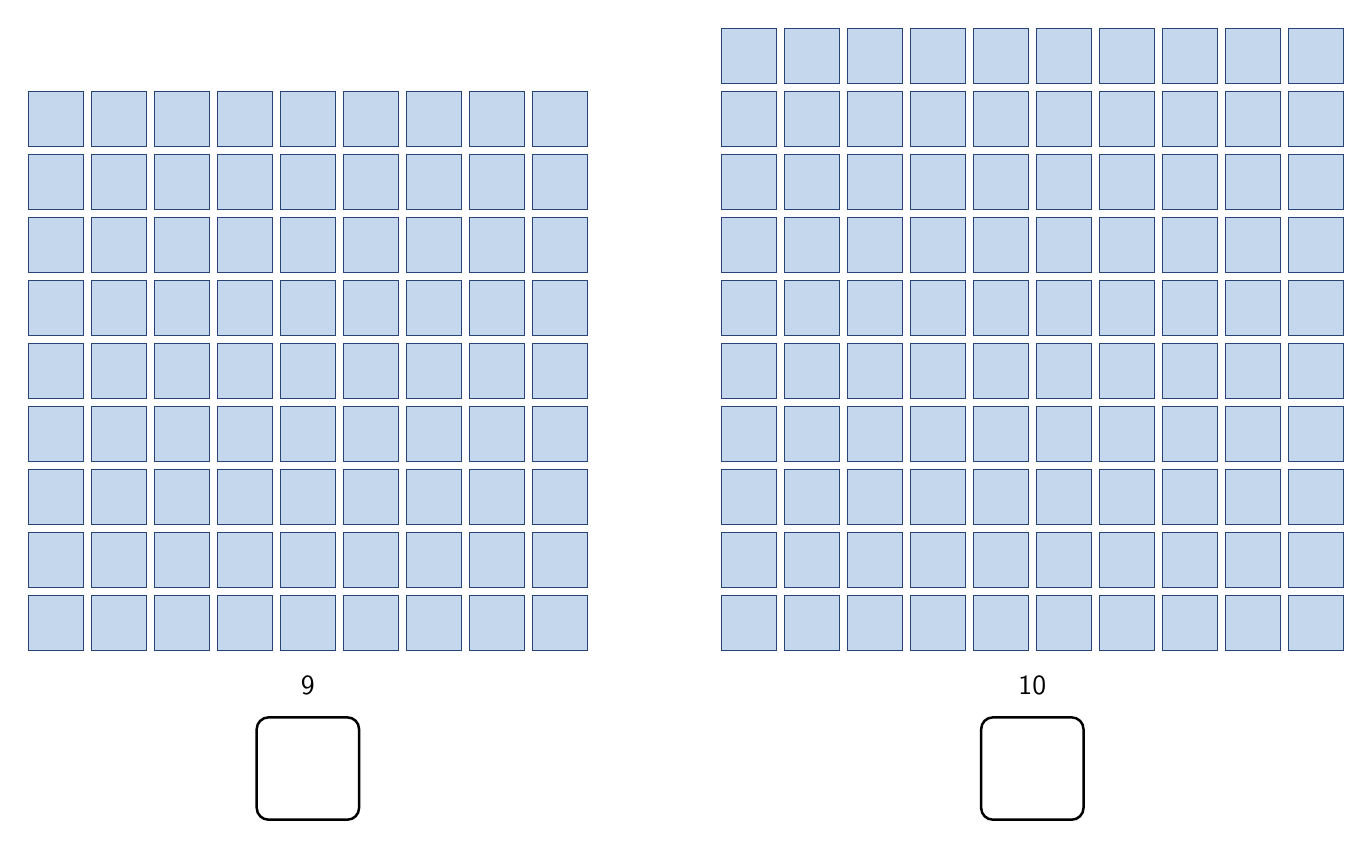
\begin{tikzpicture}[x=1mm,y=1mm]
\filldraw[fill=tilefill!45,draw=tileline,line width=0.4pt] (0.48,0.48) rectangle (7.52,7.52);
\filldraw[fill=tilefill!45,draw=tileline,line width=0.4pt] (0.48,8.48) rectangle (7.52,15.52);
\filldraw[fill=tilefill!45,draw=tileline,line width=0.4pt] (0.48,16.48) rectangle (7.52,23.52);
\filldraw[fill=tilefill!45,draw=tileline,line width=0.4pt] (0.48,24.48) rectangle (7.52,31.52);
\filldraw[fill=tilefill!45,draw=tileline,line width=0.4pt] (0.48,32.48) rectangle (7.52,39.52);
\filldraw[fill=tilefill!45,draw=tileline,line width=0.4pt] (0.48,40.48) rectangle (7.52,47.52);
\filldraw[fill=tilefill!45,draw=tileline,line width=0.4pt] (0.48,48.48) rectangle (7.52,55.52);
\filldraw[fill=tilefill!45,draw=tileline,line width=0.4pt] (0.48,56.48) rectangle (7.52,63.52);
\filldraw[fill=tilefill!45,draw=tileline,line width=0.4pt] (0.48,64.48) rectangle (7.52,71.52);
\filldraw[fill=tilefill!45,draw=tileline,line width=0.4pt] (8.48,0.48) rectangle (15.52,7.52);
\filldraw[fill=tilefill!45,draw=tileline,line width=0.4pt] (8.48,8.48) rectangle (15.52,15.52);
\filldraw[fill=tilefill!45,draw=tileline,line width=0.4pt] (8.48,16.48) rectangle (15.52,23.52);
\filldraw[fill=tilefill!45,draw=tileline,line width=0.4pt] (8.48,24.48) rectangle (15.52,31.52);
\filldraw[fill=tilefill!45,draw=tileline,line width=0.4pt] (8.48,32.48) rectangle (15.52,39.52);
\filldraw[fill=tilefill!45,draw=tileline,line width=0.4pt] (8.48,40.48) rectangle (15.52,47.52);
\filldraw[fill=tilefill!45,draw=tileline,line width=0.4pt] (8.48,48.48) rectangle (15.52,55.52);
\filldraw[fill=tilefill!45,draw=tileline,line width=0.4pt] (8.48,56.48) rectangle (15.52,63.52);
\filldraw[fill=tilefill!45,draw=tileline,line width=0.4pt] (8.48,64.48) rectangle (15.52,71.52);
\filldraw[fill=tilefill!45,draw=tileline,line width=0.4pt] (16.48,0.48) rectangle (23.52,7.52);
\filldraw[fill=tilefill!45,draw=tileline,line width=0.4pt] (16.48,8.48) rectangle (23.52,15.52);
\filldraw[fill=tilefill!45,draw=tileline,line width=0.4pt] (16.48,16.48) rectangle (23.52,23.52);
\filldraw[fill=tilefill!45,draw=tileline,line width=0.4pt] (16.48,24.48) rectangle (23.52,31.52);
\filldraw[fill=tilefill!45,draw=tileline,line width=0.4pt] (16.48,32.48) rectangle (23.52,39.52);
\filldraw[fill=tilefill!45,draw=tileline,line width=0.4pt] (16.48,40.48) rectangle (23.52,47.52);
\filldraw[fill=tilefill!45,draw=tileline,line width=0.4pt] (16.48,48.48) rectangle (23.52,55.52);
\filldraw[fill=tilefill!45,draw=tileline,line width=0.4pt] (16.48,56.48) rectangle (23.52,63.52);
\filldraw[fill=tilefill!45,draw=tileline,line width=0.4pt] (16.48,64.48) rectangle (23.52,71.52);
\filldraw[fill=tilefill!45,draw=tileline,line width=0.4pt] (24.48,0.48) rectangle (31.52,7.52);
\filldraw[fill=tilefill!45,draw=tileline,line width=0.4pt] (24.48,8.48) rectangle (31.52,15.52);
\filldraw[fill=tilefill!45,draw=tileline,line width=0.4pt] (24.48,16.48) rectangle (31.52,23.52);
\filldraw[fill=tilefill!45,draw=tileline,line width=0.4pt] (24.48,24.48) rectangle (31.52,31.52);
\filldraw[fill=tilefill!45,draw=tileline,line width=0.4pt] (24.48,32.48) rectangle (31.52,39.52);
\filldraw[fill=tilefill!45,draw=tileline,line width=0.4pt] (24.48,40.48) rectangle (31.52,47.52);
\filldraw[fill=tilefill!45,draw=tileline,line width=0.4pt] (24.48,48.48) rectangle (31.52,55.52);
\filldraw[fill=tilefill!45,draw=tileline,line width=0.4pt] (24.48,56.48) rectangle (31.52,63.52);
\filldraw[fill=tilefill!45,draw=tileline,line width=0.4pt] (24.48,64.48) rectangle (31.52,71.52);
\filldraw[fill=tilefill!45,draw=tileline,line width=0.4pt] (32.48,0.48) rectangle (39.52,7.52);
\filldraw[fill=tilefill!45,draw=tileline,line width=0.4pt] (32.48,8.48) rectangle (39.52,15.52);
\filldraw[fill=tilefill!45,draw=tileline,line width=0.4pt] (32.48,16.48) rectangle (39.52,23.52);
\filldraw[fill=tilefill!45,draw=tileline,line width=0.4pt] (32.48,24.48) rectangle (39.52,31.52);
\filldraw[fill=tilefill!45,draw=tileline,line width=0.4pt] (32.48,32.48) rectangle (39.52,39.52);
\filldraw[fill=tilefill!45,draw=tileline,line width=0.4pt] (32.48,40.48) rectangle (39.52,47.52);
\filldraw[fill=tilefill!45,draw=tileline,line width=0.4pt] (32.48,48.48) rectangle (39.52,55.52);
\filldraw[fill=tilefill!45,draw=tileline,line width=0.4pt] (32.48,56.48) rectangle (39.52,63.52);
\filldraw[fill=tilefill!45,draw=tileline,line width=0.4pt] (32.48,64.48) rectangle (39.52,71.52);
\filldraw[fill=tilefill!45,draw=tileline,line width=0.4pt] (40.48,0.48) rectangle (47.52,7.52);
\filldraw[fill=tilefill!45,draw=tileline,line width=0.4pt] (40.48,8.48) rectangle (47.52,15.52);
\filldraw[fill=tilefill!45,draw=tileline,line width=0.4pt] (40.48,16.48) rectangle (47.52,23.52);
\filldraw[fill=tilefill!45,draw=tileline,line width=0.4pt] (40.48,24.48) rectangle (47.52,31.52);
\filldraw[fill=tilefill!45,draw=tileline,line width=0.4pt] (40.48,32.48) rectangle (47.52,39.52);
\filldraw[fill=tilefill!45,draw=tileline,line width=0.4pt] (40.48,40.48) rectangle (47.52,47.52);
\filldraw[fill=tilefill!45,draw=tileline,line width=0.4pt] (40.48,48.48) rectangle (47.52,55.52);
\filldraw[fill=tilefill!45,draw=tileline,line width=0.4pt] (40.48,56.48) rectangle (47.52,63.52);
\filldraw[fill=tilefill!45,draw=tileline,line width=0.4pt] (40.48,64.48) rectangle (47.52,71.52);
\filldraw[fill=tilefill!45,draw=tileline,line width=0.4pt] (48.48,0.48) rectangle (55.52,7.52);
\filldraw[fill=tilefill!45,draw=tileline,line width=0.4pt] (48.48,8.48) rectangle (55.52,15.52);
\filldraw[fill=tilefill!45,draw=tileline,line width=0.4pt] (48.48,16.48) rectangle (55.52,23.52);
\filldraw[fill=tilefill!45,draw=tileline,line width=0.4pt] (48.48,24.48) rectangle (55.52,31.52);
\filldraw[fill=tilefill!45,draw=tileline,line width=0.4pt] (48.48,32.48) rectangle (55.52,39.52);
\filldraw[fill=tilefill!45,draw=tileline,line width=0.4pt] (48.48,40.48) rectangle (55.52,47.52);
\filldraw[fill=tilefill!45,draw=tileline,line width=0.4pt] (48.48,48.48) rectangle (55.52,55.52);
\filldraw[fill=tilefill!45,draw=tileline,line width=0.4pt] (48.48,56.48) rectangle (55.52,63.52);
\filldraw[fill=tilefill!45,draw=tileline,line width=0.4pt] (48.48,64.48) rectangle (55.52,71.52);
\filldraw[fill=tilefill!45,draw=tileline,line width=0.4pt] (56.48,0.48) rectangle (63.52,7.52);
\filldraw[fill=tilefill!45,draw=tileline,line width=0.4pt] (56.48,8.48) rectangle (63.52,15.52);
\filldraw[fill=tilefill!45,draw=tileline,line width=0.4pt] (56.48,16.48) rectangle (63.52,23.52);
\filldraw[fill=tilefill!45,draw=tileline,line width=0.4pt] (56.48,24.48) rectangle (63.52,31.52);
\filldraw[fill=tilefill!45,draw=tileline,line width=0.4pt] (56.48,32.48) rectangle (63.52,39.52);
\filldraw[fill=tilefill!45,draw=tileline,line width=0.4pt] (56.48,40.48) rectangle (63.52,47.52);
\filldraw[fill=tilefill!45,draw=tileline,line width=0.4pt] (56.48,48.48) rectangle (63.52,55.52);
\filldraw[fill=tilefill!45,draw=tileline,line width=0.4pt] (56.48,56.48) rectangle (63.52,63.52);
\filldraw[fill=tilefill!45,draw=tileline,line width=0.4pt] (56.48,64.48) rectangle (63.52,71.52);
\filldraw[fill=tilefill!45,draw=tileline,line width=0.4pt] (64.48,0.48) rectangle (71.52,7.52);
\filldraw[fill=tilefill!45,draw=tileline,line width=0.4pt] (64.48,8.48) rectangle (71.52,15.52);
\filldraw[fill=tilefill!45,draw=tileline,line width=0.4pt] (64.48,16.48) rectangle (71.52,23.52);
\filldraw[fill=tilefill!45,draw=tileline,line width=0.4pt] (64.48,24.48) rectangle (71.52,31.52);
\filldraw[fill=tilefill!45,draw=tileline,line width=0.4pt] (64.48,32.48) rectangle (71.52,39.52);
\filldraw[fill=tilefill!45,draw=tileline,line width=0.4pt] (64.48,40.48) rectangle (71.52,47.52);
\filldraw[fill=tilefill!45,draw=tileline,line width=0.4pt] (64.48,48.48) rectangle (71.52,55.52);
\filldraw[fill=tilefill!45,draw=tileline,line width=0.4pt] (64.48,56.48) rectangle (71.52,63.52);
\filldraw[fill=tilefill!45,draw=tileline,line width=0.4pt] (64.48,64.48) rectangle (71.52,71.52);
\node[lab] at (36,-4) {9};
\draw[wbox] (29.5,-21) rectangle (42.5,-8);
\filldraw[fill=tilefill!45,draw=tileline,line width=0.4pt] (88.48,0.48) rectangle (95.52,7.52);
\filldraw[fill=tilefill!45,draw=tileline,line width=0.4pt] (88.48,8.48) rectangle (95.52,15.52);
\filldraw[fill=tilefill!45,draw=tileline,line width=0.4pt] (88.48,16.48) rectangle (95.52,23.52);
\filldraw[fill=tilefill!45,draw=tileline,line width=0.4pt] (88.48,24.48) rectangle (95.52,31.52);
\filldraw[fill=tilefill!45,draw=tileline,line width=0.4pt] (88.48,32.48) rectangle (95.52,39.52);
\filldraw[fill=tilefill!45,draw=tileline,line width=0.4pt] (88.48,40.48) rectangle (95.52,47.52);
\filldraw[fill=tilefill!45,draw=tileline,line width=0.4pt] (88.48,48.48) rectangle (95.52,55.52);
\filldraw[fill=tilefill!45,draw=tileline,line width=0.4pt] (88.48,56.48) rectangle (95.52,63.52);
\filldraw[fill=tilefill!45,draw=tileline,line width=0.4pt] (88.48,64.48) rectangle (95.52,71.52);
\filldraw[fill=tilefill!45,draw=tileline,line width=0.4pt] (88.48,72.48) rectangle (95.52,79.52);
\filldraw[fill=tilefill!45,draw=tileline,line width=0.4pt] (96.48,0.48) rectangle (103.52,7.52);
\filldraw[fill=tilefill!45,draw=tileline,line width=0.4pt] (96.48,8.48) rectangle (103.52,15.52);
\filldraw[fill=tilefill!45,draw=tileline,line width=0.4pt] (96.48,16.48) rectangle (103.52,23.52);
\filldraw[fill=tilefill!45,draw=tileline,line width=0.4pt] (96.48,24.48) rectangle (103.52,31.52);
\filldraw[fill=tilefill!45,draw=tileline,line width=0.4pt] (96.48,32.48) rectangle (103.52,39.52);
\filldraw[fill=tilefill!45,draw=tileline,line width=0.4pt] (96.48,40.48) rectangle (103.52,47.52);
\filldraw[fill=tilefill!45,draw=tileline,line width=0.4pt] (96.48,48.48) rectangle (103.52,55.52);
\filldraw[fill=tilefill!45,draw=tileline,line width=0.4pt] (96.48,56.48) rectangle (103.52,63.52);
\filldraw[fill=tilefill!45,draw=tileline,line width=0.4pt] (96.48,64.48) rectangle (103.52,71.52);
\filldraw[fill=tilefill!45,draw=tileline,line width=0.4pt] (96.48,72.48) rectangle (103.52,79.52);
\filldraw[fill=tilefill!45,draw=tileline,line width=0.4pt] (104.48,0.48) rectangle (111.52,7.52);
\filldraw[fill=tilefill!45,draw=tileline,line width=0.4pt] (104.48,8.48) rectangle (111.52,15.52);
\filldraw[fill=tilefill!45,draw=tileline,line width=0.4pt] (104.48,16.48) rectangle (111.52,23.52);
\filldraw[fill=tilefill!45,draw=tileline,line width=0.4pt] (104.48,24.48) rectangle (111.52,31.52);
\filldraw[fill=tilefill!45,draw=tileline,line width=0.4pt] (104.48,32.48) rectangle (111.52,39.52);
\filldraw[fill=tilefill!45,draw=tileline,line width=0.4pt] (104.48,40.48) rectangle (111.52,47.52);
\filldraw[fill=tilefill!45,draw=tileline,line width=0.4pt] (104.48,48.48) rectangle (111.52,55.52);
\filldraw[fill=tilefill!45,draw=tileline,line width=0.4pt] (104.48,56.48) rectangle (111.52,63.52);
\filldraw[fill=tilefill!45,draw=tileline,line width=0.4pt] (104.48,64.48) rectangle (111.52,71.52);
\filldraw[fill=tilefill!45,draw=tileline,line width=0.4pt] (104.48,72.48) rectangle (111.52,79.52);
\filldraw[fill=tilefill!45,draw=tileline,line width=0.4pt] (112.48,0.48) rectangle (119.52,7.52);
\filldraw[fill=tilefill!45,draw=tileline,line width=0.4pt] (112.48,8.48) rectangle (119.52,15.52);
\filldraw[fill=tilefill!45,draw=tileline,line width=0.4pt] (112.48,16.48) rectangle (119.52,23.52);
\filldraw[fill=tilefill!45,draw=tileline,line width=0.4pt] (112.48,24.48) rectangle (119.52,31.52);
\filldraw[fill=tilefill!45,draw=tileline,line width=0.4pt] (112.48,32.48) rectangle (119.52,39.52);
\filldraw[fill=tilefill!45,draw=tileline,line width=0.4pt] (112.48,40.48) rectangle (119.52,47.52);
\filldraw[fill=tilefill!45,draw=tileline,line width=0.4pt] (112.48,48.48) rectangle (119.52,55.52);
\filldraw[fill=tilefill!45,draw=tileline,line width=0.4pt] (112.48,56.48) rectangle (119.52,63.52);
\filldraw[fill=tilefill!45,draw=tileline,line width=0.4pt] (112.48,64.48) rectangle (119.52,71.52);
\filldraw[fill=tilefill!45,draw=tileline,line width=0.4pt] (112.48,72.48) rectangle (119.52,79.52);
\filldraw[fill=tilefill!45,draw=tileline,line width=0.4pt] (120.48,0.48) rectangle (127.52,7.52);
\filldraw[fill=tilefill!45,draw=tileline,line width=0.4pt] (120.48,8.48) rectangle (127.52,15.52);
\filldraw[fill=tilefill!45,draw=tileline,line width=0.4pt] (120.48,16.48) rectangle (127.52,23.52);
\filldraw[fill=tilefill!45,draw=tileline,line width=0.4pt] (120.48,24.48) rectangle (127.52,31.52);
\filldraw[fill=tilefill!45,draw=tileline,line width=0.4pt] (120.48,32.48) rectangle (127.52,39.52);
\filldraw[fill=tilefill!45,draw=tileline,line width=0.4pt] (120.48,40.48) rectangle (127.52,47.52);
\filldraw[fill=tilefill!45,draw=tileline,line width=0.4pt] (120.48,48.48) rectangle (127.52,55.52);
\filldraw[fill=tilefill!45,draw=tileline,line width=0.4pt] (120.48,56.48) rectangle (127.52,63.52);
\filldraw[fill=tilefill!45,draw=tileline,line width=0.4pt] (120.48,64.48) rectangle (127.52,71.52);
\filldraw[fill=tilefill!45,draw=tileline,line width=0.4pt] (120.48,72.48) rectangle (127.52,79.52);
\filldraw[fill=tilefill!45,draw=tileline,line width=0.4pt] (128.48,0.48) rectangle (135.52,7.52);
\filldraw[fill=tilefill!45,draw=tileline,line width=0.4pt] (128.48,8.48) rectangle (135.52,15.52);
\filldraw[fill=tilefill!45,draw=tileline,line width=0.4pt] (128.48,16.48) rectangle (135.52,23.52);
\filldraw[fill=tilefill!45,draw=tileline,line width=0.4pt] (128.48,24.48) rectangle (135.52,31.52);
\filldraw[fill=tilefill!45,draw=tileline,line width=0.4pt] (128.48,32.48) rectangle (135.52,39.52);
\filldraw[fill=tilefill!45,draw=tileline,line width=0.4pt] (128.48,40.48) rectangle (135.52,47.52);
\filldraw[fill=tilefill!45,draw=tileline,line width=0.4pt] (128.48,48.48) rectangle (135.52,55.52);
\filldraw[fill=tilefill!45,draw=tileline,line width=0.4pt] (128.48,56.48) rectangle (135.52,63.52);
\filldraw[fill=tilefill!45,draw=tileline,line width=0.4pt] (128.48,64.48) rectangle (135.52,71.52);
\filldraw[fill=tilefill!45,draw=tileline,line width=0.4pt] (128.48,72.48) rectangle (135.52,79.52);
\filldraw[fill=tilefill!45,draw=tileline,line width=0.4pt] (136.48,0.48) rectangle (143.52,7.52);
\filldraw[fill=tilefill!45,draw=tileline,line width=0.4pt] (136.48,8.48) rectangle (143.52,15.52);
\filldraw[fill=tilefill!45,draw=tileline,line width=0.4pt] (136.48,16.48) rectangle (143.52,23.52);
\filldraw[fill=tilefill!45,draw=tileline,line width=0.4pt] (136.48,24.48) rectangle (143.52,31.52);
\filldraw[fill=tilefill!45,draw=tileline,line width=0.4pt] (136.48,32.48) rectangle (143.52,39.52);
\filldraw[fill=tilefill!45,draw=tileline,line width=0.4pt] (136.48,40.48) rectangle (143.52,47.52);
\filldraw[fill=tilefill!45,draw=tileline,line width=0.4pt] (136.48,48.48) rectangle (143.52,55.52);
\filldraw[fill=tilefill!45,draw=tileline,line width=0.4pt] (136.48,56.48) rectangle (143.52,63.52);
\filldraw[fill=tilefill!45,draw=tileline,line width=0.4pt] (136.48,64.48) rectangle (143.52,71.52);
\filldraw[fill=tilefill!45,draw=tileline,line width=0.4pt] (136.48,72.48) rectangle (143.52,79.52);
\filldraw[fill=tilefill!45,draw=tileline,line width=0.4pt] (144.48,0.48) rectangle (151.52,7.52);
\filldraw[fill=tilefill!45,draw=tileline,line width=0.4pt] (144.48,8.48) rectangle (151.52,15.52);
\filldraw[fill=tilefill!45,draw=tileline,line width=0.4pt] (144.48,16.48) rectangle (151.52,23.52);
\filldraw[fill=tilefill!45,draw=tileline,line width=0.4pt] (144.48,24.48) rectangle (151.52,31.52);
\filldraw[fill=tilefill!45,draw=tileline,line width=0.4pt] (144.48,32.48) rectangle (151.52,39.52);
\filldraw[fill=tilefill!45,draw=tileline,line width=0.4pt] (144.48,40.48) rectangle (151.52,47.52);
\filldraw[fill=tilefill!45,draw=tileline,line width=0.4pt] (144.48,48.48) rectangle (151.52,55.52);
\filldraw[fill=tilefill!45,draw=tileline,line width=0.4pt] (144.48,56.48) rectangle (151.52,63.52);
\filldraw[fill=tilefill!45,draw=tileline,line width=0.4pt] (144.48,64.48) rectangle (151.52,71.52);
\filldraw[fill=tilefill!45,draw=tileline,line width=0.4pt] (144.48,72.48) rectangle (151.52,79.52);
\filldraw[fill=tilefill!45,draw=tileline,line width=0.4pt] (152.48,0.48) rectangle (159.52,7.52);
\filldraw[fill=tilefill!45,draw=tileline,line width=0.4pt] (152.48,8.48) rectangle (159.52,15.52);
\filldraw[fill=tilefill!45,draw=tileline,line width=0.4pt] (152.48,16.48) rectangle (159.52,23.52);
\filldraw[fill=tilefill!45,draw=tileline,line width=0.4pt] (152.48,24.48) rectangle (159.52,31.52);
\filldraw[fill=tilefill!45,draw=tileline,line width=0.4pt] (152.48,32.48) rectangle (159.52,39.52);
\filldraw[fill=tilefill!45,draw=tileline,line width=0.4pt] (152.48,40.48) rectangle (159.52,47.52);
\filldraw[fill=tilefill!45,draw=tileline,line width=0.4pt] (152.48,48.48) rectangle (159.52,55.52);
\filldraw[fill=tilefill!45,draw=tileline,line width=0.4pt] (152.48,56.48) rectangle (159.52,63.52);
\filldraw[fill=tilefill!45,draw=tileline,line width=0.4pt] (152.48,64.48) rectangle (159.52,71.52);
\filldraw[fill=tilefill!45,draw=tileline,line width=0.4pt] (152.48,72.48) rectangle (159.52,79.52);
\filldraw[fill=tilefill!45,draw=tileline,line width=0.4pt] (160.48,0.48) rectangle (167.52,7.52);
\filldraw[fill=tilefill!45,draw=tileline,line width=0.4pt] (160.48,8.48) rectangle (167.52,15.52);
\filldraw[fill=tilefill!45,draw=tileline,line width=0.4pt] (160.48,16.48) rectangle (167.52,23.52);
\filldraw[fill=tilefill!45,draw=tileline,line width=0.4pt] (160.48,24.48) rectangle (167.52,31.52);
\filldraw[fill=tilefill!45,draw=tileline,line width=0.4pt] (160.48,32.48) rectangle (167.52,39.52);
\filldraw[fill=tilefill!45,draw=tileline,line width=0.4pt] (160.48,40.48) rectangle (167.52,47.52);
\filldraw[fill=tilefill!45,draw=tileline,line width=0.4pt] (160.48,48.48) rectangle (167.52,55.52);
\filldraw[fill=tilefill!45,draw=tileline,line width=0.4pt] (160.48,56.48) rectangle (167.52,63.52);
\filldraw[fill=tilefill!45,draw=tileline,line width=0.4pt] (160.48,64.48) rectangle (167.52,71.52);
\filldraw[fill=tilefill!45,draw=tileline,line width=0.4pt] (160.48,72.48) rectangle (167.52,79.52);
\node[lab] at (128,-4) {10};
\draw[wbox] (121.5,-21) rectangle (134.5,-8);
\end{tikzpicture}\par}
\vfill
\newpage
\prob{9}Build each square on the table from the middle out, one ring at a time, and take away groups of~8. What does each square leave?\par
\vspace{8mm}
\noindent\hspace*{3mm}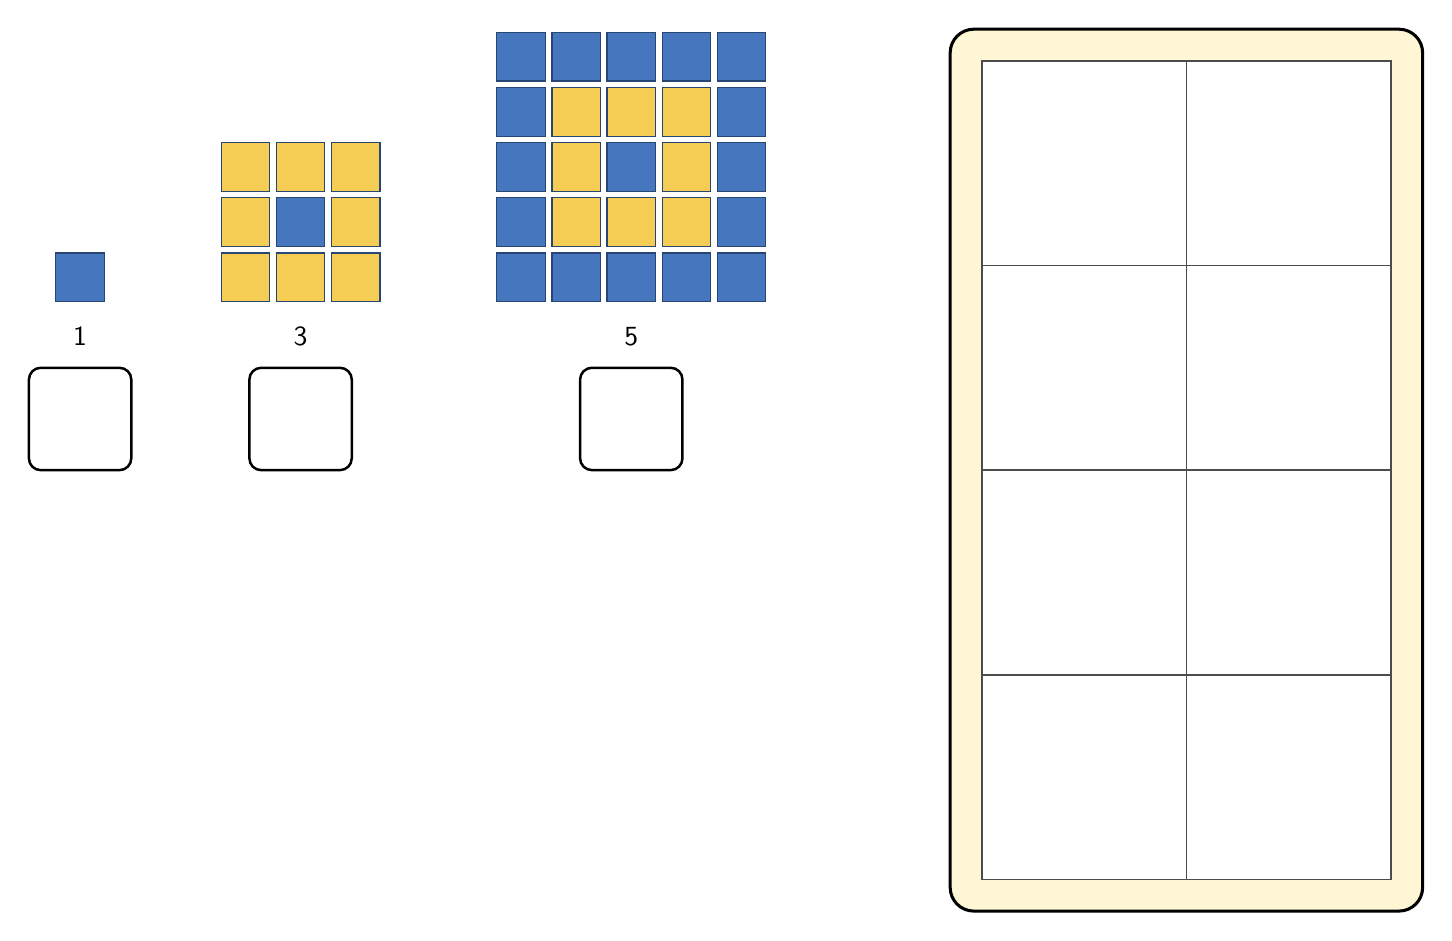
\begin{tikzpicture}[x=1mm,y=1mm]
\filldraw[fill=ringA,draw=tileline,line width=0.45pt] (0.42,0.42) rectangle (6.58,6.58);
\node[lab] at (3.5,-4) {1};
\draw[wbox] (-3,-21) rectangle (10,-8);
\filldraw[fill=ringB,draw=tileline,line width=0.45pt] (21.42,0.42) rectangle (27.58,6.58);
\filldraw[fill=ringB,draw=tileline,line width=0.45pt] (21.42,7.42) rectangle (27.58,13.58);
\filldraw[fill=ringB,draw=tileline,line width=0.45pt] (21.42,14.42) rectangle (27.58,20.58);
\filldraw[fill=ringB,draw=tileline,line width=0.45pt] (28.42,0.42) rectangle (34.58,6.58);
\filldraw[fill=ringA,draw=tileline,line width=0.45pt] (28.42,7.42) rectangle (34.58,13.58);
\filldraw[fill=ringB,draw=tileline,line width=0.45pt] (28.42,14.42) rectangle (34.58,20.58);
\filldraw[fill=ringB,draw=tileline,line width=0.45pt] (35.42,0.42) rectangle (41.58,6.58);
\filldraw[fill=ringB,draw=tileline,line width=0.45pt] (35.42,7.42) rectangle (41.58,13.58);
\filldraw[fill=ringB,draw=tileline,line width=0.45pt] (35.42,14.42) rectangle (41.58,20.58);
\node[lab] at (31.5,-4) {3};
\draw[wbox] (25,-21) rectangle (38,-8);
\filldraw[fill=ringA,draw=tileline,line width=0.45pt] (56.42,0.42) rectangle (62.58,6.58);
\filldraw[fill=ringA,draw=tileline,line width=0.45pt] (56.42,7.42) rectangle (62.58,13.58);
\filldraw[fill=ringA,draw=tileline,line width=0.45pt] (56.42,14.42) rectangle (62.58,20.58);
\filldraw[fill=ringA,draw=tileline,line width=0.45pt] (56.42,21.42) rectangle (62.58,27.58);
\filldraw[fill=ringA,draw=tileline,line width=0.45pt] (56.42,28.42) rectangle (62.58,34.58);
\filldraw[fill=ringA,draw=tileline,line width=0.45pt] (63.42,0.42) rectangle (69.58,6.58);
\filldraw[fill=ringB,draw=tileline,line width=0.45pt] (63.42,7.42) rectangle (69.58,13.58);
\filldraw[fill=ringB,draw=tileline,line width=0.45pt] (63.42,14.42) rectangle (69.58,20.58);
\filldraw[fill=ringB,draw=tileline,line width=0.45pt] (63.42,21.42) rectangle (69.58,27.58);
\filldraw[fill=ringA,draw=tileline,line width=0.45pt] (63.42,28.42) rectangle (69.58,34.58);
\filldraw[fill=ringA,draw=tileline,line width=0.45pt] (70.42,0.42) rectangle (76.58,6.58);
\filldraw[fill=ringB,draw=tileline,line width=0.45pt] (70.42,7.42) rectangle (76.58,13.58);
\filldraw[fill=ringA,draw=tileline,line width=0.45pt] (70.42,14.42) rectangle (76.58,20.58);
\filldraw[fill=ringB,draw=tileline,line width=0.45pt] (70.42,21.42) rectangle (76.58,27.58);
\filldraw[fill=ringA,draw=tileline,line width=0.45pt] (70.42,28.42) rectangle (76.58,34.58);
\filldraw[fill=ringA,draw=tileline,line width=0.45pt] (77.42,0.42) rectangle (83.58,6.58);
\filldraw[fill=ringB,draw=tileline,line width=0.45pt] (77.42,7.42) rectangle (83.58,13.58);
\filldraw[fill=ringB,draw=tileline,line width=0.45pt] (77.42,14.42) rectangle (83.58,20.58);
\filldraw[fill=ringB,draw=tileline,line width=0.45pt] (77.42,21.42) rectangle (83.58,27.58);
\filldraw[fill=ringA,draw=tileline,line width=0.45pt] (77.42,28.42) rectangle (83.58,34.58);
\filldraw[fill=ringA,draw=tileline,line width=0.45pt] (84.42,0.42) rectangle (90.58,6.58);
\filldraw[fill=ringA,draw=tileline,line width=0.45pt] (84.42,7.42) rectangle (90.58,13.58);
\filldraw[fill=ringA,draw=tileline,line width=0.45pt] (84.42,14.42) rectangle (90.58,20.58);
\filldraw[fill=ringA,draw=tileline,line width=0.45pt] (84.42,21.42) rectangle (90.58,27.58);
\filldraw[fill=ringA,draw=tileline,line width=0.45pt] (84.42,28.42) rectangle (90.58,34.58);
\node[lab] at (73.5,-4) {5};
\draw[wbox] (67,-21) rectangle (80,-8);
\filldraw[fill=cardfill,draw=black,line width=1.1pt,rounded corners=3mm] (114,-77) rectangle (174,35);
\filldraw[fill=white,draw=black!70,line width=0.6pt] (118,-73) rectangle (144,-47);
\filldraw[fill=white,draw=black!70,line width=0.6pt] (118,-47) rectangle (144,-21);
\filldraw[fill=white,draw=black!70,line width=0.6pt] (118,-21) rectangle (144,5);
\filldraw[fill=white,draw=black!70,line width=0.6pt] (118,5) rectangle (144,31);
\filldraw[fill=white,draw=black!70,line width=0.6pt] (144,-73) rectangle (170,-47);
\filldraw[fill=white,draw=black!70,line width=0.6pt] (144,-47) rectangle (170,-21);
\filldraw[fill=white,draw=black!70,line width=0.6pt] (144,-21) rectangle (170,5);
\filldraw[fill=white,draw=black!70,line width=0.6pt] (144,5) rectangle (170,31);
\end{tikzpicture}\par
\vfill
\newpage
\prob{10}What would this square leave in groups of~8? Explain how you know.\par
\vspace{8mm}
\noindent\hspace*{3mm}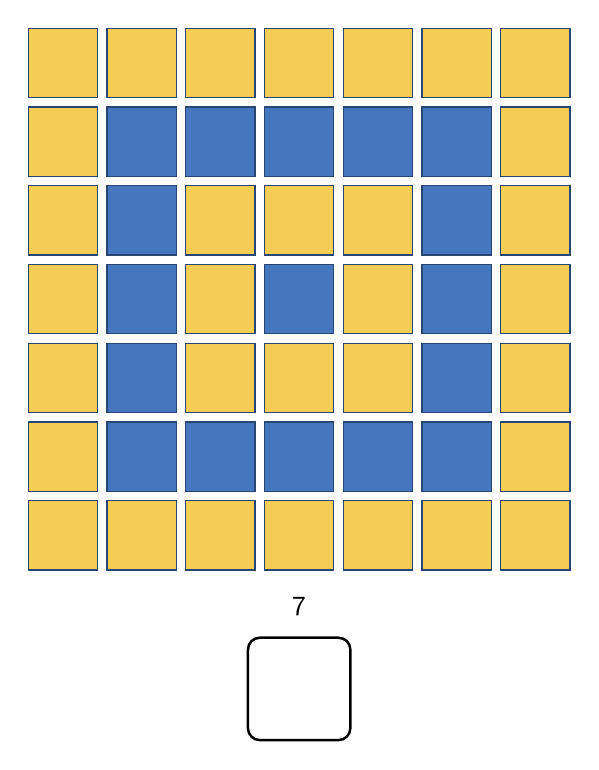
\begin{tikzpicture}[x=1mm,y=1mm]
\filldraw[fill=ringB,draw=tileline,line width=0.45pt] (0.6,0.6) rectangle (9.4,9.4);
\filldraw[fill=ringB,draw=tileline,line width=0.45pt] (0.6,10.6) rectangle (9.4,19.4);
\filldraw[fill=ringB,draw=tileline,line width=0.45pt] (0.6,20.6) rectangle (9.4,29.4);
\filldraw[fill=ringB,draw=tileline,line width=0.45pt] (0.6,30.6) rectangle (9.4,39.4);
\filldraw[fill=ringB,draw=tileline,line width=0.45pt] (0.6,40.6) rectangle (9.4,49.4);
\filldraw[fill=ringB,draw=tileline,line width=0.45pt] (0.6,50.6) rectangle (9.4,59.4);
\filldraw[fill=ringB,draw=tileline,line width=0.45pt] (0.6,60.6) rectangle (9.4,69.4);
\filldraw[fill=ringB,draw=tileline,line width=0.45pt] (10.6,0.6) rectangle (19.4,9.4);
\filldraw[fill=ringA,draw=tileline,line width=0.45pt] (10.6,10.6) rectangle (19.4,19.4);
\filldraw[fill=ringA,draw=tileline,line width=0.45pt] (10.6,20.6) rectangle (19.4,29.4);
\filldraw[fill=ringA,draw=tileline,line width=0.45pt] (10.6,30.6) rectangle (19.4,39.4);
\filldraw[fill=ringA,draw=tileline,line width=0.45pt] (10.6,40.6) rectangle (19.4,49.4);
\filldraw[fill=ringA,draw=tileline,line width=0.45pt] (10.6,50.6) rectangle (19.4,59.4);
\filldraw[fill=ringB,draw=tileline,line width=0.45pt] (10.6,60.6) rectangle (19.4,69.4);
\filldraw[fill=ringB,draw=tileline,line width=0.45pt] (20.6,0.6) rectangle (29.4,9.4);
\filldraw[fill=ringA,draw=tileline,line width=0.45pt] (20.6,10.6) rectangle (29.4,19.4);
\filldraw[fill=ringB,draw=tileline,line width=0.45pt] (20.6,20.6) rectangle (29.4,29.4);
\filldraw[fill=ringB,draw=tileline,line width=0.45pt] (20.6,30.6) rectangle (29.4,39.4);
\filldraw[fill=ringB,draw=tileline,line width=0.45pt] (20.6,40.6) rectangle (29.4,49.4);
\filldraw[fill=ringA,draw=tileline,line width=0.45pt] (20.6,50.6) rectangle (29.4,59.4);
\filldraw[fill=ringB,draw=tileline,line width=0.45pt] (20.6,60.6) rectangle (29.4,69.4);
\filldraw[fill=ringB,draw=tileline,line width=0.45pt] (30.6,0.6) rectangle (39.4,9.4);
\filldraw[fill=ringA,draw=tileline,line width=0.45pt] (30.6,10.6) rectangle (39.4,19.4);
\filldraw[fill=ringB,draw=tileline,line width=0.45pt] (30.6,20.6) rectangle (39.4,29.4);
\filldraw[fill=ringA,draw=tileline,line width=0.45pt] (30.6,30.6) rectangle (39.4,39.4);
\filldraw[fill=ringB,draw=tileline,line width=0.45pt] (30.6,40.6) rectangle (39.4,49.4);
\filldraw[fill=ringA,draw=tileline,line width=0.45pt] (30.6,50.6) rectangle (39.4,59.4);
\filldraw[fill=ringB,draw=tileline,line width=0.45pt] (30.6,60.6) rectangle (39.4,69.4);
\filldraw[fill=ringB,draw=tileline,line width=0.45pt] (40.6,0.6) rectangle (49.4,9.4);
\filldraw[fill=ringA,draw=tileline,line width=0.45pt] (40.6,10.6) rectangle (49.4,19.4);
\filldraw[fill=ringB,draw=tileline,line width=0.45pt] (40.6,20.6) rectangle (49.4,29.4);
\filldraw[fill=ringB,draw=tileline,line width=0.45pt] (40.6,30.6) rectangle (49.4,39.4);
\filldraw[fill=ringB,draw=tileline,line width=0.45pt] (40.6,40.6) rectangle (49.4,49.4);
\filldraw[fill=ringA,draw=tileline,line width=0.45pt] (40.6,50.6) rectangle (49.4,59.4);
\filldraw[fill=ringB,draw=tileline,line width=0.45pt] (40.6,60.6) rectangle (49.4,69.4);
\filldraw[fill=ringB,draw=tileline,line width=0.45pt] (50.6,0.6) rectangle (59.4,9.4);
\filldraw[fill=ringA,draw=tileline,line width=0.45pt] (50.6,10.6) rectangle (59.4,19.4);
\filldraw[fill=ringA,draw=tileline,line width=0.45pt] (50.6,20.6) rectangle (59.4,29.4);
\filldraw[fill=ringA,draw=tileline,line width=0.45pt] (50.6,30.6) rectangle (59.4,39.4);
\filldraw[fill=ringA,draw=tileline,line width=0.45pt] (50.6,40.6) rectangle (59.4,49.4);
\filldraw[fill=ringA,draw=tileline,line width=0.45pt] (50.6,50.6) rectangle (59.4,59.4);
\filldraw[fill=ringB,draw=tileline,line width=0.45pt] (50.6,60.6) rectangle (59.4,69.4);
\filldraw[fill=ringB,draw=tileline,line width=0.45pt] (60.6,0.6) rectangle (69.4,9.4);
\filldraw[fill=ringB,draw=tileline,line width=0.45pt] (60.6,10.6) rectangle (69.4,19.4);
\filldraw[fill=ringB,draw=tileline,line width=0.45pt] (60.6,20.6) rectangle (69.4,29.4);
\filldraw[fill=ringB,draw=tileline,line width=0.45pt] (60.6,30.6) rectangle (69.4,39.4);
\filldraw[fill=ringB,draw=tileline,line width=0.45pt] (60.6,40.6) rectangle (69.4,49.4);
\filldraw[fill=ringB,draw=tileline,line width=0.45pt] (60.6,50.6) rectangle (69.4,59.4);
\filldraw[fill=ringB,draw=tileline,line width=0.45pt] (60.6,60.6) rectangle (69.4,69.4);
\node[lab] at (35,-4) {7};
\draw[wbox] (28.5,-21) rectangle (41.5,-8);
\end{tikzpicture}\par
\vfill
\newpage
\prob{11}Play Problem~2 again with these cards and groups of~8.\par
\vspace{7mm}
{\centering 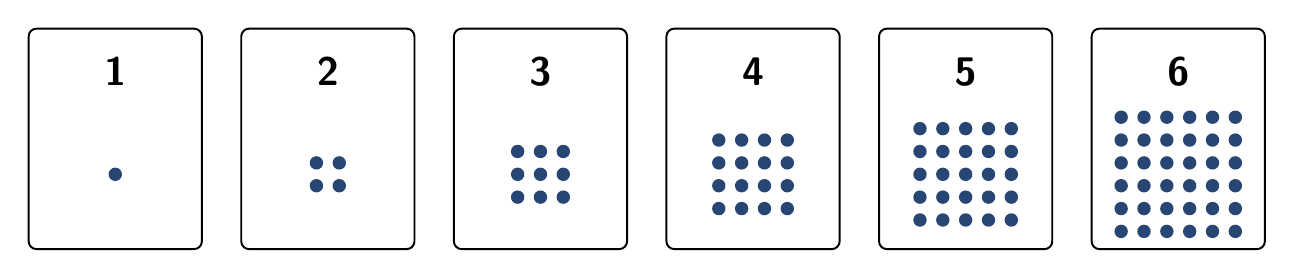
\begin{tikzpicture}[x=1mm,y=1mm]
\draw[line width=0.7pt,rounded corners=1mm] (0,0) rectangle (22,28);
\node[font=\Large\bfseries] at (11,22.5) {1};
\fill[tileline] (11,9.5) circle (0.85);
\draw[line width=0.7pt,rounded corners=1mm] (27,0) rectangle (49,28);
\node[font=\Large\bfseries] at (38,22.5) {2};
\fill[tileline] (36.55,8.05) circle (0.85);
\fill[tileline] (36.55,10.95) circle (0.85);
\fill[tileline] (39.45,8.05) circle (0.85);
\fill[tileline] (39.45,10.95) circle (0.85);
\draw[line width=0.7pt,rounded corners=1mm] (54,0) rectangle (76,28);
\node[font=\Large\bfseries] at (65,22.5) {3};
\fill[tileline] (62.1,6.6) circle (0.85);
\fill[tileline] (62.1,9.5) circle (0.85);
\fill[tileline] (62.1,12.4) circle (0.85);
\fill[tileline] (65,6.6) circle (0.85);
\fill[tileline] (65,9.5) circle (0.85);
\fill[tileline] (65,12.4) circle (0.85);
\fill[tileline] (67.9,6.6) circle (0.85);
\fill[tileline] (67.9,9.5) circle (0.85);
\fill[tileline] (67.9,12.4) circle (0.85);
\draw[line width=0.7pt,rounded corners=1mm] (81,0) rectangle (103,28);
\node[font=\Large\bfseries] at (92,22.5) {4};
\fill[tileline] (87.65,5.15) circle (0.85);
\fill[tileline] (87.65,8.05) circle (0.85);
\fill[tileline] (87.65,10.95) circle (0.85);
\fill[tileline] (87.65,13.85) circle (0.85);
\fill[tileline] (90.55,5.15) circle (0.85);
\fill[tileline] (90.55,8.05) circle (0.85);
\fill[tileline] (90.55,10.95) circle (0.85);
\fill[tileline] (90.55,13.85) circle (0.85);
\fill[tileline] (93.45,5.15) circle (0.85);
\fill[tileline] (93.45,8.05) circle (0.85);
\fill[tileline] (93.45,10.95) circle (0.85);
\fill[tileline] (93.45,13.85) circle (0.85);
\fill[tileline] (96.35,5.15) circle (0.85);
\fill[tileline] (96.35,8.05) circle (0.85);
\fill[tileline] (96.35,10.95) circle (0.85);
\fill[tileline] (96.35,13.85) circle (0.85);
\draw[line width=0.7pt,rounded corners=1mm] (108,0) rectangle (130,28);
\node[font=\Large\bfseries] at (119,22.5) {5};
\fill[tileline] (113.2,3.7) circle (0.85);
\fill[tileline] (113.2,6.6) circle (0.85);
\fill[tileline] (113.2,9.5) circle (0.85);
\fill[tileline] (113.2,12.4) circle (0.85);
\fill[tileline] (113.2,15.3) circle (0.85);
\fill[tileline] (116.1,3.7) circle (0.85);
\fill[tileline] (116.1,6.6) circle (0.85);
\fill[tileline] (116.1,9.5) circle (0.85);
\fill[tileline] (116.1,12.4) circle (0.85);
\fill[tileline] (116.1,15.3) circle (0.85);
\fill[tileline] (119,3.7) circle (0.85);
\fill[tileline] (119,6.6) circle (0.85);
\fill[tileline] (119,9.5) circle (0.85);
\fill[tileline] (119,12.4) circle (0.85);
\fill[tileline] (119,15.3) circle (0.85);
\fill[tileline] (121.9,3.7) circle (0.85);
\fill[tileline] (121.9,6.6) circle (0.85);
\fill[tileline] (121.9,9.5) circle (0.85);
\fill[tileline] (121.9,12.4) circle (0.85);
\fill[tileline] (121.9,15.3) circle (0.85);
\fill[tileline] (124.8,3.7) circle (0.85);
\fill[tileline] (124.8,6.6) circle (0.85);
\fill[tileline] (124.8,9.5) circle (0.85);
\fill[tileline] (124.8,12.4) circle (0.85);
\fill[tileline] (124.8,15.3) circle (0.85);
\draw[line width=0.7pt,rounded corners=1mm] (135,0) rectangle (157,28);
\node[font=\Large\bfseries] at (146,22.5) {6};
\fill[tileline] (138.75,2.25) circle (0.85);
\fill[tileline] (138.75,5.15) circle (0.85);
\fill[tileline] (138.75,8.05) circle (0.85);
\fill[tileline] (138.75,10.95) circle (0.85);
\fill[tileline] (138.75,13.85) circle (0.85);
\fill[tileline] (138.75,16.75) circle (0.85);
\fill[tileline] (141.65,2.25) circle (0.85);
\fill[tileline] (141.65,5.15) circle (0.85);
\fill[tileline] (141.65,8.05) circle (0.85);
\fill[tileline] (141.65,10.95) circle (0.85);
\fill[tileline] (141.65,13.85) circle (0.85);
\fill[tileline] (141.65,16.75) circle (0.85);
\fill[tileline] (144.55,2.25) circle (0.85);
\fill[tileline] (144.55,5.15) circle (0.85);
\fill[tileline] (144.55,8.05) circle (0.85);
\fill[tileline] (144.55,10.95) circle (0.85);
\fill[tileline] (144.55,13.85) circle (0.85);
\fill[tileline] (144.55,16.75) circle (0.85);
\fill[tileline] (147.45,2.25) circle (0.85);
\fill[tileline] (147.45,5.15) circle (0.85);
\fill[tileline] (147.45,8.05) circle (0.85);
\fill[tileline] (147.45,10.95) circle (0.85);
\fill[tileline] (147.45,13.85) circle (0.85);
\fill[tileline] (147.45,16.75) circle (0.85);
\fill[tileline] (150.35,2.25) circle (0.85);
\fill[tileline] (150.35,5.15) circle (0.85);
\fill[tileline] (150.35,8.05) circle (0.85);
\fill[tileline] (150.35,10.95) circle (0.85);
\fill[tileline] (150.35,13.85) circle (0.85);
\fill[tileline] (150.35,16.75) circle (0.85);
\fill[tileline] (153.25,2.25) circle (0.85);
\fill[tileline] (153.25,5.15) circle (0.85);
\fill[tileline] (153.25,8.05) circle (0.85);
\fill[tileline] (153.25,10.95) circle (0.85);
\fill[tileline] (153.25,13.85) circle (0.85);
\fill[tileline] (153.25,16.75) circle (0.85);
\end{tikzpicture}\par}
\vspace{10mm}
\noindent\hspace*{3mm}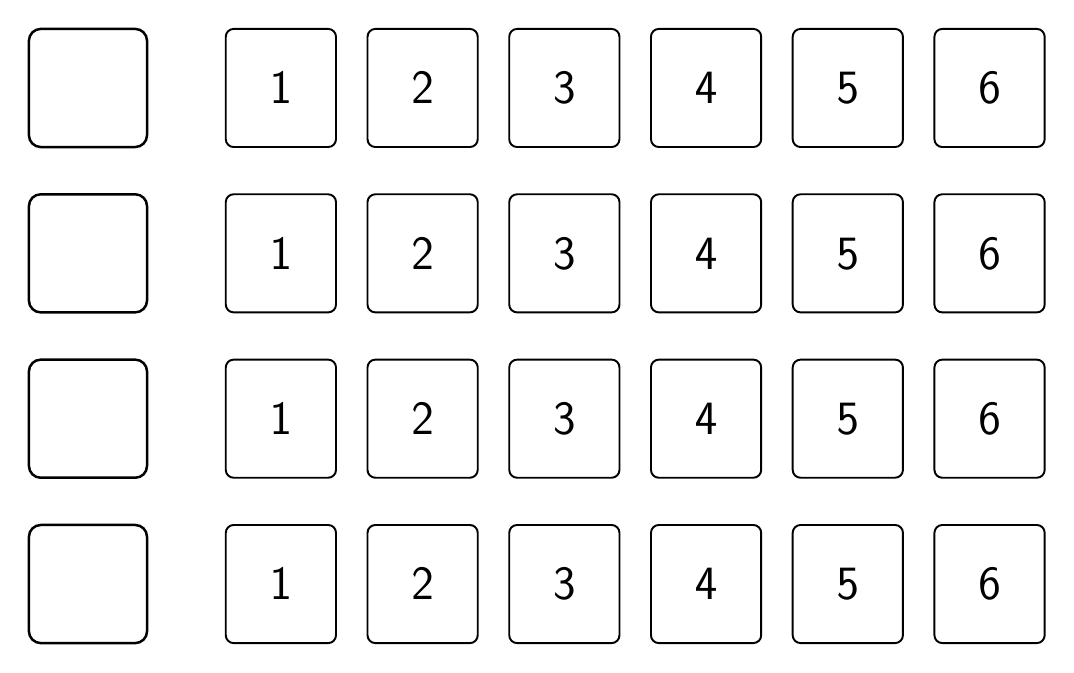
\begin{tikzpicture}[x=1mm,y=1mm]
\draw[wbox] (0,-15) rectangle (15,0);
\draw[line width=0.7pt,rounded corners=1mm] (25,-15) rectangle (39,0);
\node[font=\LARGE] at (32,-7.5) {1};
\draw[line width=0.7pt,rounded corners=1mm] (43,-15) rectangle (57,0);
\node[font=\LARGE] at (50,-7.5) {2};
\draw[line width=0.7pt,rounded corners=1mm] (61,-15) rectangle (75,0);
\node[font=\LARGE] at (68,-7.5) {3};
\draw[line width=0.7pt,rounded corners=1mm] (79,-15) rectangle (93,0);
\node[font=\LARGE] at (86,-7.5) {4};
\draw[line width=0.7pt,rounded corners=1mm] (97,-15) rectangle (111,0);
\node[font=\LARGE] at (104,-7.5) {5};
\draw[line width=0.7pt,rounded corners=1mm] (115,-15) rectangle (129,0);
\node[font=\LARGE] at (122,-7.5) {6};
\draw[wbox] (0,-36) rectangle (15,-21);
\draw[line width=0.7pt,rounded corners=1mm] (25,-36) rectangle (39,-21);
\node[font=\LARGE] at (32,-28.5) {1};
\draw[line width=0.7pt,rounded corners=1mm] (43,-36) rectangle (57,-21);
\node[font=\LARGE] at (50,-28.5) {2};
\draw[line width=0.7pt,rounded corners=1mm] (61,-36) rectangle (75,-21);
\node[font=\LARGE] at (68,-28.5) {3};
\draw[line width=0.7pt,rounded corners=1mm] (79,-36) rectangle (93,-21);
\node[font=\LARGE] at (86,-28.5) {4};
\draw[line width=0.7pt,rounded corners=1mm] (97,-36) rectangle (111,-21);
\node[font=\LARGE] at (104,-28.5) {5};
\draw[line width=0.7pt,rounded corners=1mm] (115,-36) rectangle (129,-21);
\node[font=\LARGE] at (122,-28.5) {6};
\draw[wbox] (0,-57) rectangle (15,-42);
\draw[line width=0.7pt,rounded corners=1mm] (25,-57) rectangle (39,-42);
\node[font=\LARGE] at (32,-49.5) {1};
\draw[line width=0.7pt,rounded corners=1mm] (43,-57) rectangle (57,-42);
\node[font=\LARGE] at (50,-49.5) {2};
\draw[line width=0.7pt,rounded corners=1mm] (61,-57) rectangle (75,-42);
\node[font=\LARGE] at (68,-49.5) {3};
\draw[line width=0.7pt,rounded corners=1mm] (79,-57) rectangle (93,-42);
\node[font=\LARGE] at (86,-49.5) {4};
\draw[line width=0.7pt,rounded corners=1mm] (97,-57) rectangle (111,-42);
\node[font=\LARGE] at (104,-49.5) {5};
\draw[line width=0.7pt,rounded corners=1mm] (115,-57) rectangle (129,-42);
\node[font=\LARGE] at (122,-49.5) {6};
\draw[wbox] (0,-78) rectangle (15,-63);
\draw[line width=0.7pt,rounded corners=1mm] (25,-78) rectangle (39,-63);
\node[font=\LARGE] at (32,-70.5) {1};
\draw[line width=0.7pt,rounded corners=1mm] (43,-78) rectangle (57,-63);
\node[font=\LARGE] at (50,-70.5) {2};
\draw[line width=0.7pt,rounded corners=1mm] (61,-78) rectangle (75,-63);
\node[font=\LARGE] at (68,-70.5) {3};
\draw[line width=0.7pt,rounded corners=1mm] (79,-78) rectangle (93,-63);
\node[font=\LARGE] at (86,-70.5) {4};
\draw[line width=0.7pt,rounded corners=1mm] (97,-78) rectangle (111,-63);
\node[font=\LARGE] at (104,-70.5) {5};
\draw[line width=0.7pt,rounded corners=1mm] (115,-78) rectangle (129,-63);
\node[font=\LARGE] at (122,-70.5) {6};
\end{tikzpicture}\par
\vspace{8mm}
\noindent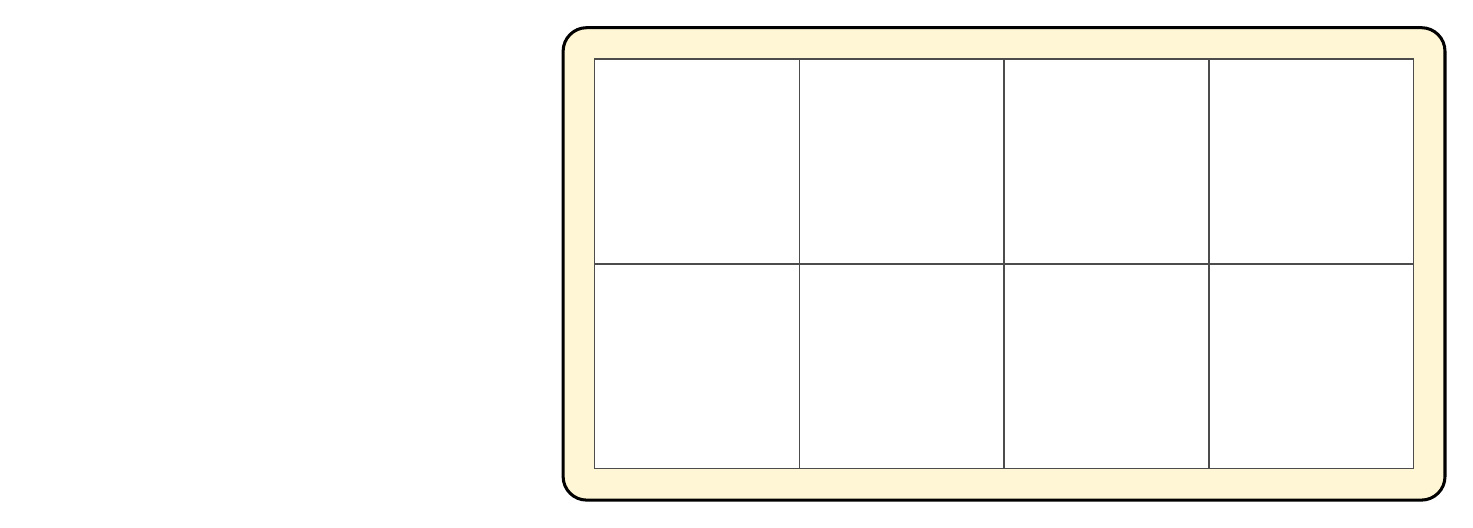
\begin{tikzpicture}[x=1mm,y=1mm]
\useasboundingbox (0,0) rectangle (180,-60);
\filldraw[fill=cardfill,draw=black,line width=1.1pt,rounded corners=3mm] (68,-60) rectangle (180,0);
\filldraw[fill=white,draw=black!70,line width=0.6pt] (72,-56) rectangle (98,-30);
\filldraw[fill=white,draw=black!70,line width=0.6pt] (72,-30) rectangle (98,-4);
\filldraw[fill=white,draw=black!70,line width=0.6pt] (98,-56) rectangle (124,-30);
\filldraw[fill=white,draw=black!70,line width=0.6pt] (98,-30) rectangle (124,-4);
\filldraw[fill=white,draw=black!70,line width=0.6pt] (124,-56) rectangle (150,-30);
\filldraw[fill=white,draw=black!70,line width=0.6pt] (124,-30) rectangle (150,-4);
\filldraw[fill=white,draw=black!70,line width=0.6pt] (150,-56) rectangle (176,-30);
\filldraw[fill=white,draw=black!70,line width=0.6pt] (150,-30) rectangle (176,-4);
\end{tikzpicture}\par
\vfill
\newpage
\vspace*{6mm}
{\centering 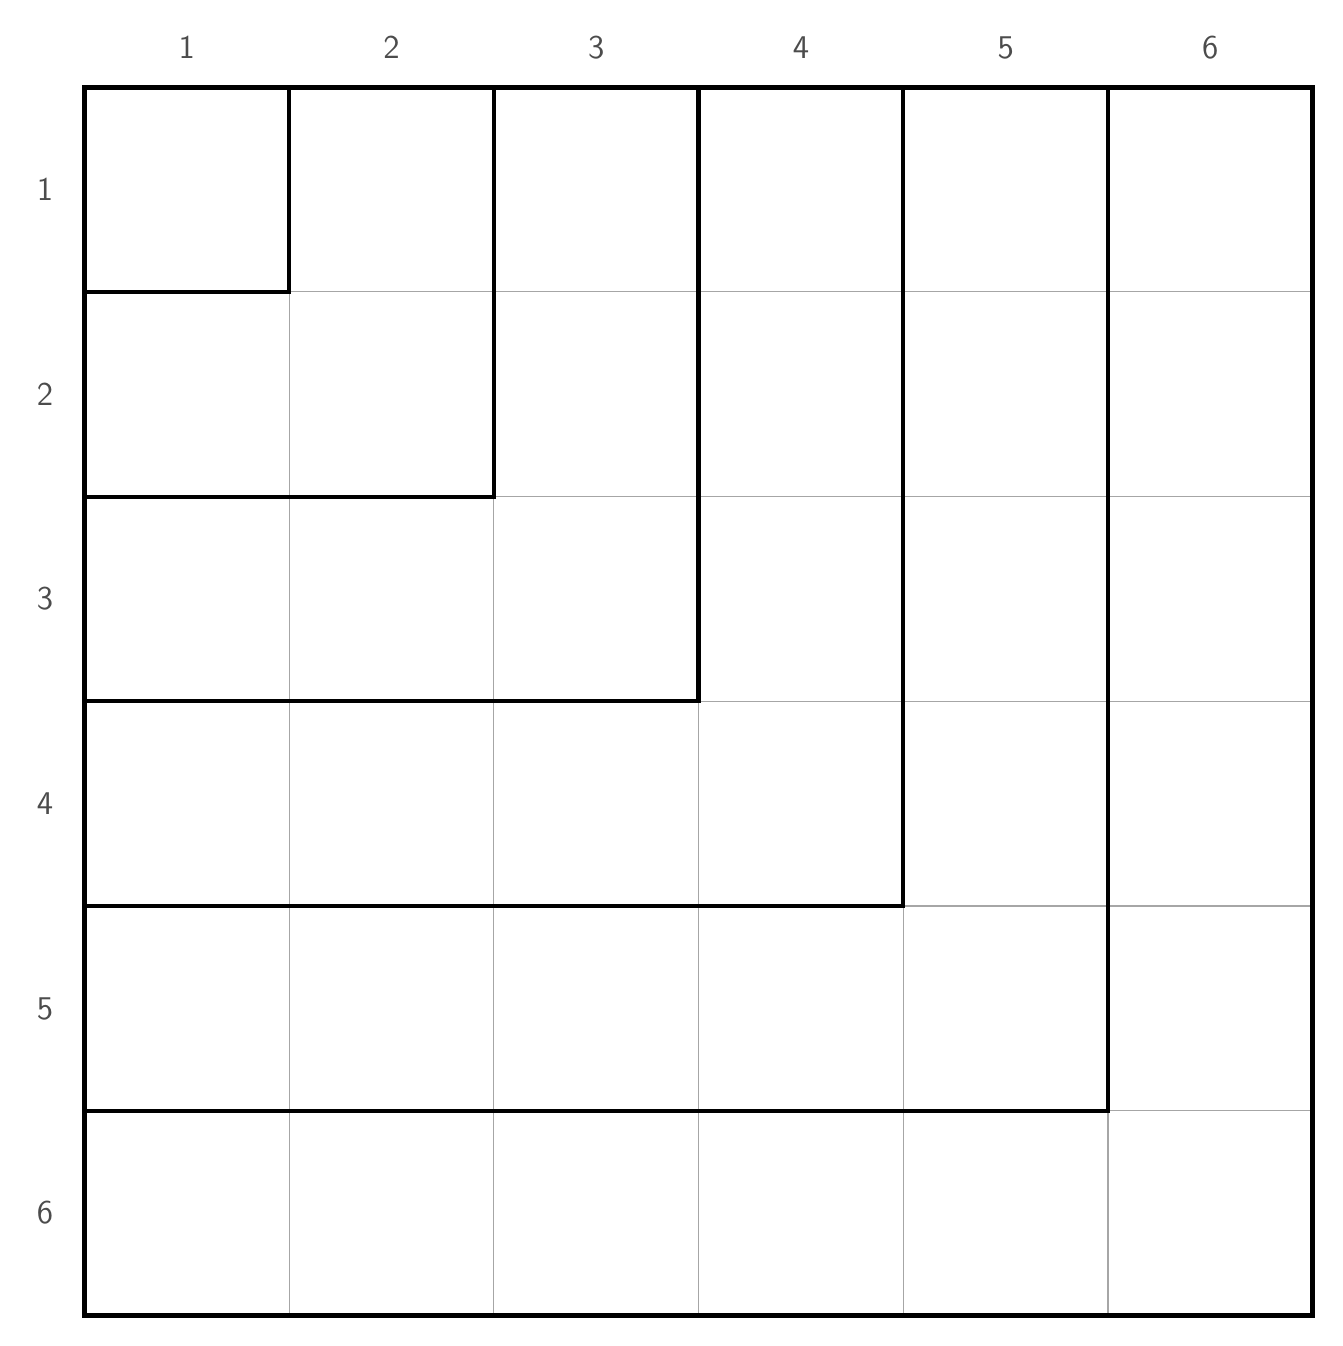
\begin{tikzpicture}[x=1mm,y=1mm]
\draw[black!35,line width=0.4pt] (26,0) -- (26,-156);
\draw[black!35,line width=0.4pt] (0,-26) -- (156,-26);
\draw[black!35,line width=0.4pt] (52,0) -- (52,-156);
\draw[black!35,line width=0.4pt] (0,-52) -- (156,-52);
\draw[black!35,line width=0.4pt] (78,0) -- (78,-156);
\draw[black!35,line width=0.4pt] (0,-78) -- (156,-78);
\draw[black!35,line width=0.4pt] (104,0) -- (104,-156);
\draw[black!35,line width=0.4pt] (0,-104) -- (156,-104);
\draw[black!35,line width=0.4pt] (130,0) -- (130,-156);
\draw[black!35,line width=0.4pt] (0,-130) -- (156,-130);
\draw[black,line width=1.5pt] (0,-26) -- (26,-26) -- (26,0);
\draw[black,line width=1.5pt] (0,-52) -- (52,-52) -- (52,0);
\draw[black,line width=1.5pt] (0,-78) -- (78,-78) -- (78,0);
\draw[black,line width=1.5pt] (0,-104) -- (104,-104) -- (104,0);
\draw[black,line width=1.5pt] (0,-130) -- (130,-130) -- (130,0);
\draw[black,line width=1.8pt] (0,0) rectangle (156,-156);
\node[font=\large,text=black!70] at (13,5) {1};
\node[font=\large,text=black!70] at (-5,-13) {1};
\node[font=\large,text=black!70] at (39,5) {2};
\node[font=\large,text=black!70] at (-5,-39) {2};
\node[font=\large,text=black!70] at (65,5) {3};
\node[font=\large,text=black!70] at (-5,-65) {3};
\node[font=\large,text=black!70] at (91,5) {4};
\node[font=\large,text=black!70] at (-5,-91) {4};
\node[font=\large,text=black!70] at (117,5) {5};
\node[font=\large,text=black!70] at (-5,-117) {5};
\node[font=\large,text=black!70] at (143,5) {6};
\node[font=\large,text=black!70] at (-5,-143) {6};
\end{tikzpicture}\par}
\vfill
\newpage
\vspace*{8mm}
{\centering 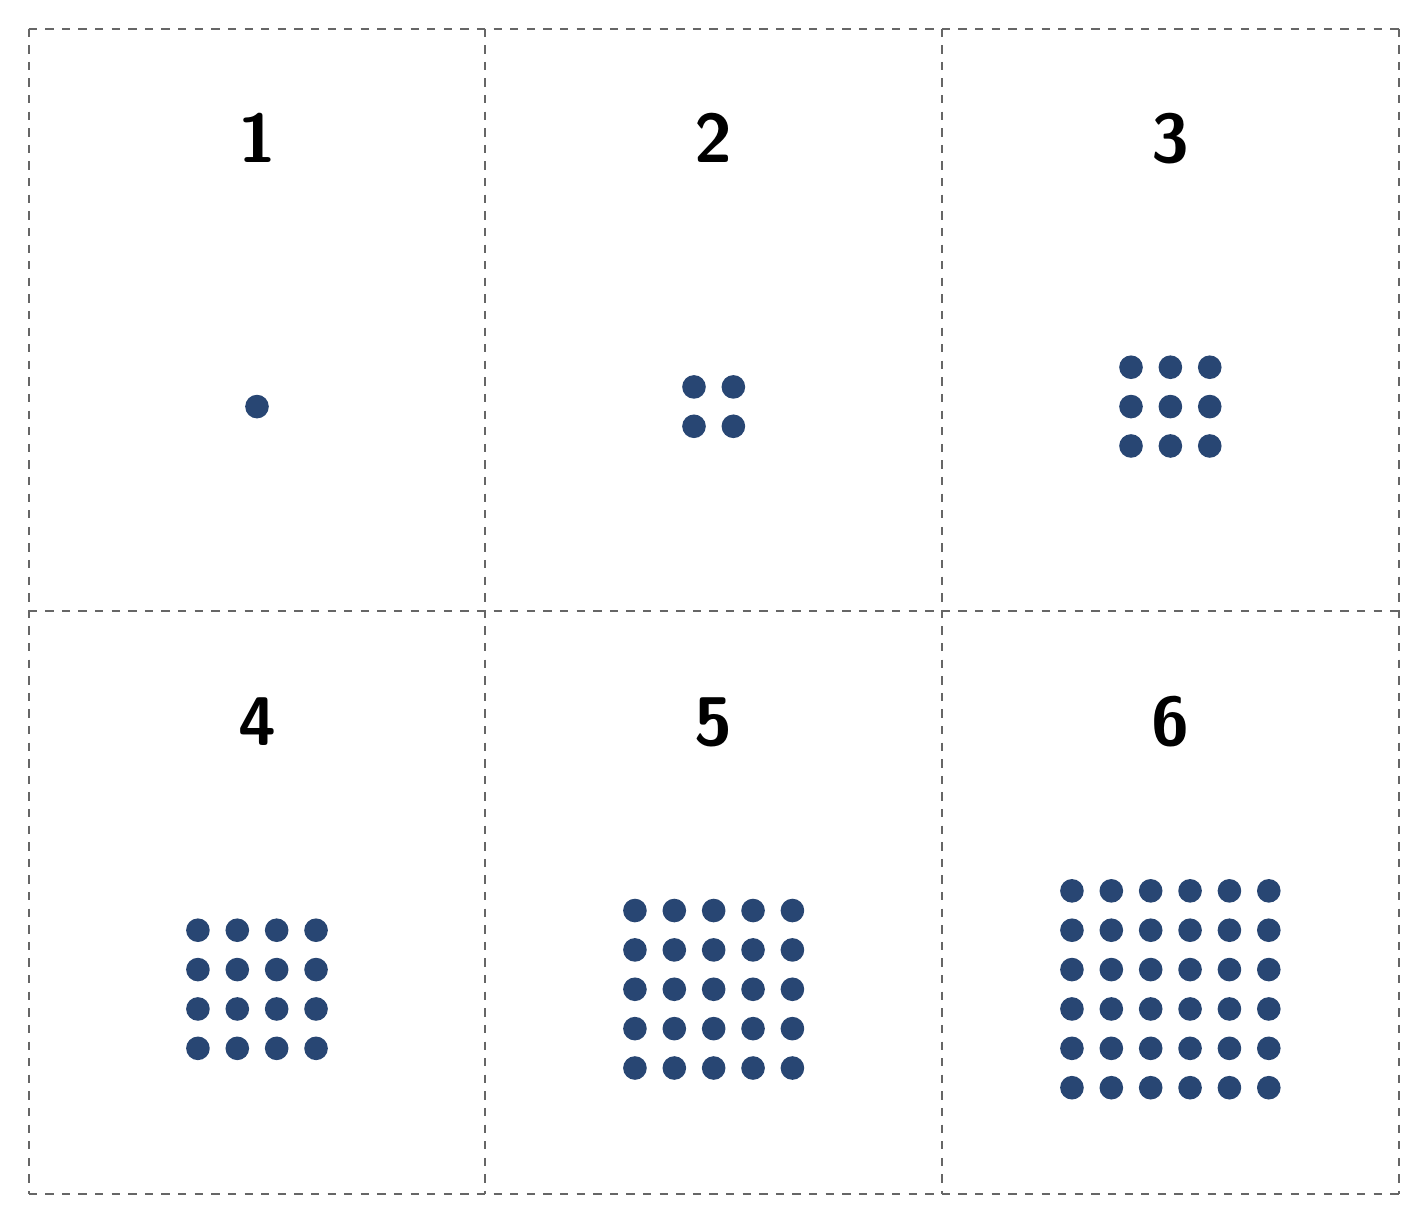
\begin{tikzpicture}[x=1mm,y=1mm]
\node[font=\fontsize{40}{44}\selectfont\bfseries] at (29,-14) {1};
\fill[tileline] (29,-48) circle (1.5);
\node[font=\fontsize{40}{44}\selectfont\bfseries] at (87,-14) {2};
\fill[tileline] (84.5,-50.5) circle (1.5);
\fill[tileline] (84.5,-45.5) circle (1.5);
\fill[tileline] (89.5,-50.5) circle (1.5);
\fill[tileline] (89.5,-45.5) circle (1.5);
\node[font=\fontsize{40}{44}\selectfont\bfseries] at (145,-14) {3};
\fill[tileline] (140,-53) circle (1.5);
\fill[tileline] (140,-48) circle (1.5);
\fill[tileline] (140,-43) circle (1.5);
\fill[tileline] (145,-53) circle (1.5);
\fill[tileline] (145,-48) circle (1.5);
\fill[tileline] (145,-43) circle (1.5);
\fill[tileline] (150,-53) circle (1.5);
\fill[tileline] (150,-48) circle (1.5);
\fill[tileline] (150,-43) circle (1.5);
\node[font=\fontsize{40}{44}\selectfont\bfseries] at (29,-88) {4};
\fill[tileline] (21.5,-129.5) circle (1.5);
\fill[tileline] (21.5,-124.5) circle (1.5);
\fill[tileline] (21.5,-119.5) circle (1.5);
\fill[tileline] (21.5,-114.5) circle (1.5);
\fill[tileline] (26.5,-129.5) circle (1.5);
\fill[tileline] (26.5,-124.5) circle (1.5);
\fill[tileline] (26.5,-119.5) circle (1.5);
\fill[tileline] (26.5,-114.5) circle (1.5);
\fill[tileline] (31.5,-129.5) circle (1.5);
\fill[tileline] (31.5,-124.5) circle (1.5);
\fill[tileline] (31.5,-119.5) circle (1.5);
\fill[tileline] (31.5,-114.5) circle (1.5);
\fill[tileline] (36.5,-129.5) circle (1.5);
\fill[tileline] (36.5,-124.5) circle (1.5);
\fill[tileline] (36.5,-119.5) circle (1.5);
\fill[tileline] (36.5,-114.5) circle (1.5);
\node[font=\fontsize{40}{44}\selectfont\bfseries] at (87,-88) {5};
\fill[tileline] (77,-132) circle (1.5);
\fill[tileline] (77,-127) circle (1.5);
\fill[tileline] (77,-122) circle (1.5);
\fill[tileline] (77,-117) circle (1.5);
\fill[tileline] (77,-112) circle (1.5);
\fill[tileline] (82,-132) circle (1.5);
\fill[tileline] (82,-127) circle (1.5);
\fill[tileline] (82,-122) circle (1.5);
\fill[tileline] (82,-117) circle (1.5);
\fill[tileline] (82,-112) circle (1.5);
\fill[tileline] (87,-132) circle (1.5);
\fill[tileline] (87,-127) circle (1.5);
\fill[tileline] (87,-122) circle (1.5);
\fill[tileline] (87,-117) circle (1.5);
\fill[tileline] (87,-112) circle (1.5);
\fill[tileline] (92,-132) circle (1.5);
\fill[tileline] (92,-127) circle (1.5);
\fill[tileline] (92,-122) circle (1.5);
\fill[tileline] (92,-117) circle (1.5);
\fill[tileline] (92,-112) circle (1.5);
\fill[tileline] (97,-132) circle (1.5);
\fill[tileline] (97,-127) circle (1.5);
\fill[tileline] (97,-122) circle (1.5);
\fill[tileline] (97,-117) circle (1.5);
\fill[tileline] (97,-112) circle (1.5);
\node[font=\fontsize{40}{44}\selectfont\bfseries] at (145,-88) {6};
\fill[tileline] (132.5,-134.5) circle (1.5);
\fill[tileline] (132.5,-129.5) circle (1.5);
\fill[tileline] (132.5,-124.5) circle (1.5);
\fill[tileline] (132.5,-119.5) circle (1.5);
\fill[tileline] (132.5,-114.5) circle (1.5);
\fill[tileline] (132.5,-109.5) circle (1.5);
\fill[tileline] (137.5,-134.5) circle (1.5);
\fill[tileline] (137.5,-129.5) circle (1.5);
\fill[tileline] (137.5,-124.5) circle (1.5);
\fill[tileline] (137.5,-119.5) circle (1.5);
\fill[tileline] (137.5,-114.5) circle (1.5);
\fill[tileline] (137.5,-109.5) circle (1.5);
\fill[tileline] (142.5,-134.5) circle (1.5);
\fill[tileline] (142.5,-129.5) circle (1.5);
\fill[tileline] (142.5,-124.5) circle (1.5);
\fill[tileline] (142.5,-119.5) circle (1.5);
\fill[tileline] (142.5,-114.5) circle (1.5);
\fill[tileline] (142.5,-109.5) circle (1.5);
\fill[tileline] (147.5,-134.5) circle (1.5);
\fill[tileline] (147.5,-129.5) circle (1.5);
\fill[tileline] (147.5,-124.5) circle (1.5);
\fill[tileline] (147.5,-119.5) circle (1.5);
\fill[tileline] (147.5,-114.5) circle (1.5);
\fill[tileline] (147.5,-109.5) circle (1.5);
\fill[tileline] (152.5,-134.5) circle (1.5);
\fill[tileline] (152.5,-129.5) circle (1.5);
\fill[tileline] (152.5,-124.5) circle (1.5);
\fill[tileline] (152.5,-119.5) circle (1.5);
\fill[tileline] (152.5,-114.5) circle (1.5);
\fill[tileline] (152.5,-109.5) circle (1.5);
\fill[tileline] (157.5,-134.5) circle (1.5);
\fill[tileline] (157.5,-129.5) circle (1.5);
\fill[tileline] (157.5,-124.5) circle (1.5);
\fill[tileline] (157.5,-119.5) circle (1.5);
\fill[tileline] (157.5,-114.5) circle (1.5);
\fill[tileline] (157.5,-109.5) circle (1.5);
\draw[dashed,line width=0.7pt,black!60] (0,0) -- (0,-148);
\draw[dashed,line width=0.7pt,black!60] (58,0) -- (58,-148);
\draw[dashed,line width=0.7pt,black!60] (116,0) -- (116,-148);
\draw[dashed,line width=0.7pt,black!60] (174,0) -- (174,-148);
\draw[dashed,line width=0.7pt,black!60] (0,0) -- (174,0);
\draw[dashed,line width=0.7pt,black!60] (0,-74) -- (174,-74);
\draw[dashed,line width=0.7pt,black!60] (0,-148) -- (174,-148);
\end{tikzpicture}\par}
\vfill

\end{document}
